% Options for packages loaded elsewhere
\PassOptionsToPackage{unicode}{hyperref}
\PassOptionsToPackage{hyphens}{url}
\PassOptionsToPackage{dvipsnames,svgnames,x11names}{xcolor}
%
\documentclass[
  letterpaper,
  DIV=11,
  numbers=noendperiod]{scrreprt}

\usepackage{amsmath,amssymb}
\usepackage{iftex}
\ifPDFTeX
  \usepackage[T1]{fontenc}
  \usepackage[utf8]{inputenc}
  \usepackage{textcomp} % provide euro and other symbols
\else % if luatex or xetex
  \usepackage{unicode-math}
  \defaultfontfeatures{Scale=MatchLowercase}
  \defaultfontfeatures[\rmfamily]{Ligatures=TeX,Scale=1}
\fi
\usepackage{lmodern}
\ifPDFTeX\else  
    % xetex/luatex font selection
\fi
% Use upquote if available, for straight quotes in verbatim environments
\IfFileExists{upquote.sty}{\usepackage{upquote}}{}
\IfFileExists{microtype.sty}{% use microtype if available
  \usepackage[]{microtype}
  \UseMicrotypeSet[protrusion]{basicmath} % disable protrusion for tt fonts
}{}
\makeatletter
\@ifundefined{KOMAClassName}{% if non-KOMA class
  \IfFileExists{parskip.sty}{%
    \usepackage{parskip}
  }{% else
    \setlength{\parindent}{0pt}
    \setlength{\parskip}{6pt plus 2pt minus 1pt}}
}{% if KOMA class
  \KOMAoptions{parskip=half}}
\makeatother
\usepackage{xcolor}
\setlength{\emergencystretch}{3em} % prevent overfull lines
\setcounter{secnumdepth}{5}
% Make \paragraph and \subparagraph free-standing
\ifx\paragraph\undefined\else
  \let\oldparagraph\paragraph
  \renewcommand{\paragraph}[1]{\oldparagraph{#1}\mbox{}}
\fi
\ifx\subparagraph\undefined\else
  \let\oldsubparagraph\subparagraph
  \renewcommand{\subparagraph}[1]{\oldsubparagraph{#1}\mbox{}}
\fi

\usepackage{color}
\usepackage{fancyvrb}
\newcommand{\VerbBar}{|}
\newcommand{\VERB}{\Verb[commandchars=\\\{\}]}
\DefineVerbatimEnvironment{Highlighting}{Verbatim}{commandchars=\\\{\}}
% Add ',fontsize=\small' for more characters per line
\usepackage{framed}
\definecolor{shadecolor}{RGB}{241,243,245}
\newenvironment{Shaded}{\begin{snugshade}}{\end{snugshade}}
\newcommand{\AlertTok}[1]{\textcolor[rgb]{0.68,0.00,0.00}{#1}}
\newcommand{\AnnotationTok}[1]{\textcolor[rgb]{0.37,0.37,0.37}{#1}}
\newcommand{\AttributeTok}[1]{\textcolor[rgb]{0.40,0.45,0.13}{#1}}
\newcommand{\BaseNTok}[1]{\textcolor[rgb]{0.68,0.00,0.00}{#1}}
\newcommand{\BuiltInTok}[1]{\textcolor[rgb]{0.00,0.23,0.31}{#1}}
\newcommand{\CharTok}[1]{\textcolor[rgb]{0.13,0.47,0.30}{#1}}
\newcommand{\CommentTok}[1]{\textcolor[rgb]{0.37,0.37,0.37}{#1}}
\newcommand{\CommentVarTok}[1]{\textcolor[rgb]{0.37,0.37,0.37}{\textit{#1}}}
\newcommand{\ConstantTok}[1]{\textcolor[rgb]{0.56,0.35,0.01}{#1}}
\newcommand{\ControlFlowTok}[1]{\textcolor[rgb]{0.00,0.23,0.31}{#1}}
\newcommand{\DataTypeTok}[1]{\textcolor[rgb]{0.68,0.00,0.00}{#1}}
\newcommand{\DecValTok}[1]{\textcolor[rgb]{0.68,0.00,0.00}{#1}}
\newcommand{\DocumentationTok}[1]{\textcolor[rgb]{0.37,0.37,0.37}{\textit{#1}}}
\newcommand{\ErrorTok}[1]{\textcolor[rgb]{0.68,0.00,0.00}{#1}}
\newcommand{\ExtensionTok}[1]{\textcolor[rgb]{0.00,0.23,0.31}{#1}}
\newcommand{\FloatTok}[1]{\textcolor[rgb]{0.68,0.00,0.00}{#1}}
\newcommand{\FunctionTok}[1]{\textcolor[rgb]{0.28,0.35,0.67}{#1}}
\newcommand{\ImportTok}[1]{\textcolor[rgb]{0.00,0.46,0.62}{#1}}
\newcommand{\InformationTok}[1]{\textcolor[rgb]{0.37,0.37,0.37}{#1}}
\newcommand{\KeywordTok}[1]{\textcolor[rgb]{0.00,0.23,0.31}{#1}}
\newcommand{\NormalTok}[1]{\textcolor[rgb]{0.00,0.23,0.31}{#1}}
\newcommand{\OperatorTok}[1]{\textcolor[rgb]{0.37,0.37,0.37}{#1}}
\newcommand{\OtherTok}[1]{\textcolor[rgb]{0.00,0.23,0.31}{#1}}
\newcommand{\PreprocessorTok}[1]{\textcolor[rgb]{0.68,0.00,0.00}{#1}}
\newcommand{\RegionMarkerTok}[1]{\textcolor[rgb]{0.00,0.23,0.31}{#1}}
\newcommand{\SpecialCharTok}[1]{\textcolor[rgb]{0.37,0.37,0.37}{#1}}
\newcommand{\SpecialStringTok}[1]{\textcolor[rgb]{0.13,0.47,0.30}{#1}}
\newcommand{\StringTok}[1]{\textcolor[rgb]{0.13,0.47,0.30}{#1}}
\newcommand{\VariableTok}[1]{\textcolor[rgb]{0.07,0.07,0.07}{#1}}
\newcommand{\VerbatimStringTok}[1]{\textcolor[rgb]{0.13,0.47,0.30}{#1}}
\newcommand{\WarningTok}[1]{\textcolor[rgb]{0.37,0.37,0.37}{\textit{#1}}}

\providecommand{\tightlist}{%
  \setlength{\itemsep}{0pt}\setlength{\parskip}{0pt}}\usepackage{longtable,booktabs,array}
\usepackage{calc} % for calculating minipage widths
% Correct order of tables after \paragraph or \subparagraph
\usepackage{etoolbox}
\makeatletter
\patchcmd\longtable{\par}{\if@noskipsec\mbox{}\fi\par}{}{}
\makeatother
% Allow footnotes in longtable head/foot
\IfFileExists{footnotehyper.sty}{\usepackage{footnotehyper}}{\usepackage{footnote}}
\makesavenoteenv{longtable}
\usepackage{graphicx}
\makeatletter
\def\maxwidth{\ifdim\Gin@nat@width>\linewidth\linewidth\else\Gin@nat@width\fi}
\def\maxheight{\ifdim\Gin@nat@height>\textheight\textheight\else\Gin@nat@height\fi}
\makeatother
% Scale images if necessary, so that they will not overflow the page
% margins by default, and it is still possible to overwrite the defaults
% using explicit options in \includegraphics[width, height, ...]{}
\setkeys{Gin}{width=\maxwidth,height=\maxheight,keepaspectratio}
% Set default figure placement to htbp
\makeatletter
\def\fps@figure{htbp}
\makeatother
% definitions for citeproc citations
\NewDocumentCommand\citeproctext{}{}
\NewDocumentCommand\citeproc{mm}{%
  \begingroup\def\citeproctext{#2}\cite{#1}\endgroup}
\makeatletter
 % allow citations to break across lines
 \let\@cite@ofmt\@firstofone
 % avoid brackets around text for \cite:
 \def\@biblabel#1{}
 \def\@cite#1#2{{#1\if@tempswa , #2\fi}}
\makeatother
\newlength{\cslhangindent}
\setlength{\cslhangindent}{1.5em}
\newlength{\csllabelwidth}
\setlength{\csllabelwidth}{3em}
\newenvironment{CSLReferences}[2] % #1 hanging-indent, #2 entry-spacing
 {\begin{list}{}{%
  \setlength{\itemindent}{0pt}
  \setlength{\leftmargin}{0pt}
  \setlength{\parsep}{0pt}
  % turn on hanging indent if param 1 is 1
  \ifodd #1
   \setlength{\leftmargin}{\cslhangindent}
   \setlength{\itemindent}{-1\cslhangindent}
  \fi
  % set entry spacing
  \setlength{\itemsep}{#2\baselineskip}}}
 {\end{list}}
\usepackage{calc}
\newcommand{\CSLBlock}[1]{\hfill\break\parbox[t]{\linewidth}{\strut\ignorespaces#1\strut}}
\newcommand{\CSLLeftMargin}[1]{\parbox[t]{\csllabelwidth}{\strut#1\strut}}
\newcommand{\CSLRightInline}[1]{\parbox[t]{\linewidth - \csllabelwidth}{\strut#1\strut}}
\newcommand{\CSLIndent}[1]{\hspace{\cslhangindent}#1}

\KOMAoption{captions}{tableheading}
\makeatletter
\@ifpackageloaded{tcolorbox}{}{\usepackage[skins,breakable]{tcolorbox}}
\@ifpackageloaded{fontawesome5}{}{\usepackage{fontawesome5}}
\definecolor{quarto-callout-color}{HTML}{909090}
\definecolor{quarto-callout-note-color}{HTML}{0758E5}
\definecolor{quarto-callout-important-color}{HTML}{CC1914}
\definecolor{quarto-callout-warning-color}{HTML}{EB9113}
\definecolor{quarto-callout-tip-color}{HTML}{00A047}
\definecolor{quarto-callout-caution-color}{HTML}{FC5300}
\definecolor{quarto-callout-color-frame}{HTML}{acacac}
\definecolor{quarto-callout-note-color-frame}{HTML}{4582ec}
\definecolor{quarto-callout-important-color-frame}{HTML}{d9534f}
\definecolor{quarto-callout-warning-color-frame}{HTML}{f0ad4e}
\definecolor{quarto-callout-tip-color-frame}{HTML}{02b875}
\definecolor{quarto-callout-caution-color-frame}{HTML}{fd7e14}
\makeatother
\makeatletter
\@ifpackageloaded{bookmark}{}{\usepackage{bookmark}}
\makeatother
\makeatletter
\@ifpackageloaded{caption}{}{\usepackage{caption}}
\AtBeginDocument{%
\ifdefined\contentsname
  \renewcommand*\contentsname{Table of contents}
\else
  \newcommand\contentsname{Table of contents}
\fi
\ifdefined\listfigurename
  \renewcommand*\listfigurename{List of Figures}
\else
  \newcommand\listfigurename{List of Figures}
\fi
\ifdefined\listtablename
  \renewcommand*\listtablename{List of Tables}
\else
  \newcommand\listtablename{List of Tables}
\fi
\ifdefined\figurename
  \renewcommand*\figurename{Figure}
\else
  \newcommand\figurename{Figure}
\fi
\ifdefined\tablename
  \renewcommand*\tablename{Table}
\else
  \newcommand\tablename{Table}
\fi
}
\@ifpackageloaded{float}{}{\usepackage{float}}
\floatstyle{ruled}
\@ifundefined{c@chapter}{\newfloat{codelisting}{h}{lop}}{\newfloat{codelisting}{h}{lop}[chapter]}
\floatname{codelisting}{Listing}
\newcommand*\listoflistings{\listof{codelisting}{List of Listings}}
\makeatother
\makeatletter
\makeatother
\makeatletter
\@ifpackageloaded{caption}{}{\usepackage{caption}}
\@ifpackageloaded{subcaption}{}{\usepackage{subcaption}}
\makeatother
\makeatletter
\@ifpackageloaded{tikz}{}{\usepackage{tikz}}
\makeatother
        \newcommand*\circled[1]{\tikz[baseline=(char.base)]{
          \node[shape=circle,draw,inner sep=1pt] (char) {{\scriptsize#1}};}}  
                  
\ifLuaTeX
  \usepackage{selnolig}  % disable illegal ligatures
\fi
\usepackage{bookmark}

\IfFileExists{xurl.sty}{\usepackage{xurl}}{} % add URL line breaks if available
\urlstyle{same} % disable monospaced font for URLs
\hypersetup{
  pdftitle={Getting Started},
  pdfauthor={David G. Oppenheimer},
  colorlinks=true,
  linkcolor={blue},
  filecolor={Maroon},
  citecolor={Blue},
  urlcolor={Blue},
  pdfcreator={LaTeX via pandoc}}

\title{Getting Started}
\author{David G. Oppenheimer}
\date{2024-10-02}

\begin{document}
\maketitle

\renewcommand*\contentsname{Table of contents}
{
\hypersetup{linkcolor=}
\setcounter{tocdepth}{2}
\tableofcontents
}
\bookmarksetup{startatroot}

\chapter*{Preface}\label{preface}
\addcontentsline{toc}{chapter}{Preface}

\markboth{Preface}{Preface}

This is a Quarto book.

To learn more about Quarto books visit
\url{https://quarto.org/docs/books}.

\begin{Shaded}
\begin{Highlighting}[]
\DecValTok{1} \SpecialCharTok{+} \DecValTok{1}
\end{Highlighting}
\end{Shaded}

\begin{verbatim}
[1] 2
\end{verbatim}

\bookmarksetup{startatroot}

\chapter{Introduction}\label{introduction}

This is a book created from markdown and executable code.

See Knuth (1984) for additional discussion of literate programming.

\begin{Shaded}
\begin{Highlighting}[]
\DecValTok{1} \SpecialCharTok{+} \DecValTok{1}
\end{Highlighting}
\end{Shaded}

\begin{verbatim}
[1] 2
\end{verbatim}

\bookmarksetup{startatroot}

\chapter{Summary}\label{summary}

In summary, this book has no content whatsoever.

\begin{Shaded}
\begin{Highlighting}[]
\DecValTok{1} \SpecialCharTok{+} \DecValTok{1}
\end{Highlighting}
\end{Shaded}

\begin{verbatim}
[1] 2
\end{verbatim}

\bookmarksetup{startatroot}

\chapter{Software Needed}\label{sec-software-needed}

\section{R and RStudio}\label{r-and-rstudio}

Go to \href{https://posit.co/download/rstudio-desktop/}{RStudio Desktop
download page} to download the R and RStudio Desktop installers.

\begin{tcolorbox}[enhanced jigsaw, left=2mm, title=\textcolor{quarto-callout-note-color}{\faInfo}\hspace{0.5em}{Note}, opacityback=0, breakable, colbacktitle=quarto-callout-note-color!10!white, colframe=quarto-callout-note-color-frame, arc=.35mm, titlerule=0mm, leftrule=.75mm, opacitybacktitle=0.6, toptitle=1mm, colback=white, toprule=.15mm, bottomtitle=1mm, rightrule=.15mm, coltitle=black, bottomrule=.15mm]

You need to install R first, then RStudio.

\end{tcolorbox}

The R link will take you to the \href{https://cran.rstudio.com/}{The
Comprehensive R Archive Network} where you can download an R installer
for your operating system.

The RStudio link will download the apropriate installer for your
operating system.

Download and launch the installers and follow the installation
instructions.

\section{Git and a GitHub Account}\label{git-and-a-github-account}

\begin{center}

\includegraphics[width=0.5\textwidth,height=\textheight]{assets/in_case_of_fire2.png}
\end{center}

What is version control?

\begin{quote}
Version control, also known as source control, is the practice of
tracking and managing changes to software code. Version control systems
are software tools that help software teams manage changes to source
code over time\footnote{from the Atlassian webpage on
  \href{https://www.atlassian.com/git/tutorials/what-is-version-control}{What
  is version control?}}.
\end{quote}

You can get all you need to know about git from the
\href{https://git-scm.com/book/en/v2}{Pro Git Book}. This is a great
introduction to version control and git.

\subsection{User Manual}\label{user-manual}

\href{https://happygitwithr.com/}{Happy Git and GitHub for the useR}

This is an excellent resource for all things Git, GitHub, and RStudio.
Use the left navigation to Quickly find relevant topics for how to
integrate Git and GitHub with RStudio.

\begin{tcolorbox}[enhanced jigsaw, left=2mm, title=\textcolor{quarto-callout-tip-color}{\faLightbulb}\hspace{0.5em}{Tip}, opacityback=0, breakable, colbacktitle=quarto-callout-tip-color!10!white, colframe=quarto-callout-tip-color-frame, arc=.35mm, titlerule=0mm, leftrule=.75mm, opacitybacktitle=0.6, toptitle=1mm, colback=white, toprule=.15mm, bottomtitle=1mm, rightrule=.15mm, coltitle=black, bottomrule=.15mm]

We will use \texttt{git} within RStudio. On macOS, RStudio will echo the
mac terminal. I am using \href{https://ohmyz.sh/}{Oh My Zsh} as my
\texttt{zsh} framework, and
\href{https://wezfurlong.org/wezterm/index.html}{Wezterm} as my terminal
emulator rather than the macOS default terminal application. I also have
the latest \texttt{git} version installed through
\href{https://brew.sh/}{Homebrew}. I installed the
\href{https://starship.rs/}{Starship} prompt (using Homebrew) to
customize my terminal environment.

This means that I need to adjust the settings in RStudio to use my
\texttt{zsh} environment. Go to \emph{Tools} → \emph{Global Options} →
\emph{Terminal} and choose \texttt{Zsh} from the drop-down menu for the
\emph{New terminals open with} option.

\end{tcolorbox}

\subsection{Git Tutorials}\label{git-tutorials}

\begin{tcolorbox}[enhanced jigsaw, left=2mm, title=\textcolor{quarto-callout-important-color}{\faExclamation}\hspace{0.5em}{Important}, opacityback=0, breakable, colbacktitle=quarto-callout-important-color!10!white, colframe=quarto-callout-important-color-frame, arc=.35mm, titlerule=0mm, leftrule=.75mm, opacitybacktitle=0.6, toptitle=1mm, colback=white, toprule=.15mm, bottomtitle=1mm, rightrule=.15mm, coltitle=black, bottomrule=.15mm]

Here are the learning objectives for the git section. After taking the
tutorials, you will be able to:

\begin{enumerate}
\def\labelenumi{\arabic{enumi}.}
\tightlist
\item
  Create a GitHub account.
\item
  Install Git on your local computer.
\item
  Create \texttt{ssh} keys to connect your local computer to GitHub.
\item
  Create a project and push it to GitHub.
\item
  Fork a project from GitHub.
\end{enumerate}

\end{tcolorbox}

\subsubsection{Videos}\label{videos}

\begin{itemize}
\tightlist
\item
  \href{https://www.youtube.com/watch?v=RGOj5yH7evk}{Git and GitHub for
  Beginners - Crash Course}
\item
  \href{https://www.youtube.com/watch?v=CvUiKWv2-C0}{Git Tutorial for
  Absolute Beginners}
\item
  \href{https://www.theserverside.com/blog/Coffee-Talk-Java-News-Stories-and-Opinions/GitHub-SSH-Key-Setup-Config-Ubuntu-Linux}{How
  to setup SSH in GitHub by example}
\item
  \href{https://www.theserverside.com/blog/Coffee-Talk-Java-News-Stories-and-Opinions/GitHub-SSH-Windows-Example}{How
  to SSH into GitHub on Windows example}
\item
  \href{https://www.freecodecamp.org/news/how-to-fork-a-github-repository/}{How
  to Fork a GitHub Repository}
\end{itemize}

\subsubsection{Text-based}\label{text-based}

\begin{itemize}
\tightlist
\item
  \href{https://www.freecodecamp.org/news/learn-the-basics-of-git-in-under-10-minutes-da548267cc91/}{Learn
  the Basics of Git in Under 10 Minutes}
\item
  \href{https://www.freecodecamp.org/news/how-to-fork-a-github-repository/}{How
  to Fork a GitHub Repository}
\item
  \href{https://docs.github.com/en/pull-requests/collaborating-with-pull-requests/working-with-forks/fork-a-repo}{Fork
  a repository}
\end{itemize}

\subsubsection{More Guides to Git}\label{more-guides-to-git}

\begin{itemize}
\tightlist
\item
  \href{https://www.atlassian.com/git/tutorials/what-is-version-control}{Introduction
  to Version Control} This is hosted by Atlassian, a company that uses
  their own cloud-based git repository called BitBucket. We will be
  using GitHub for all our work, so if you try tutorials on this site,
  remember to use \texttt{github} instead of \texttt{bitbucket} when
  connecting to the remote repository. Focus on the \emph{Beginner} and
  \emph{Getting Started} sections.
\item
  \href{https://github.com/carpentries-incubator/reproducible-publications-quarto/blob/main/setup.md}{Git
  and GitHub}
\item
  \href{https://think-like-a-git.net/sections/about-this-site.html}{An
  ``adavanced beginner'' guide to git}
\end{itemize}

\section{Install Git}\label{install-git}

\subsection{macOS and Linux}\label{macos-and-linux}

Git is pre-installed on macOS and Linux computers, but users may want to
update to the latest version.

On Macs, installation of Git is easiest using a package manager like
\href{https://brew.sh/}{Homebrew}. If you do not have Homebrew
installed, follow the instructions on the
\href{https://brew.sh/}{Homebrew homepage}. Then install Git with:

\begin{Shaded}
\begin{Highlighting}[]
\ExtensionTok{brew}\NormalTok{ install git}
\end{Highlighting}
\end{Shaded}

Check the installation by opening the terminal tab in RStudio (or use
whatever terminal you already have open) and entering:

\begin{Shaded}
\begin{Highlighting}[]
\FunctionTok{git} \AttributeTok{{-}{-}version}
\end{Highlighting}
\end{Shaded}

\subsubsection{Set the git path in
RStudio}\label{set-the-git-path-in-rstudio}

To get RStudio to use the updated Git, you need to tell RStudio where to
find the newly installed Git. First, get the path to the Git executable
by typing:

\begin{Shaded}
\begin{Highlighting}[]
\BuiltInTok{which}\NormalTok{ git}
\end{Highlighting}
\end{Shaded}

\begin{figure}[H]

{\centering 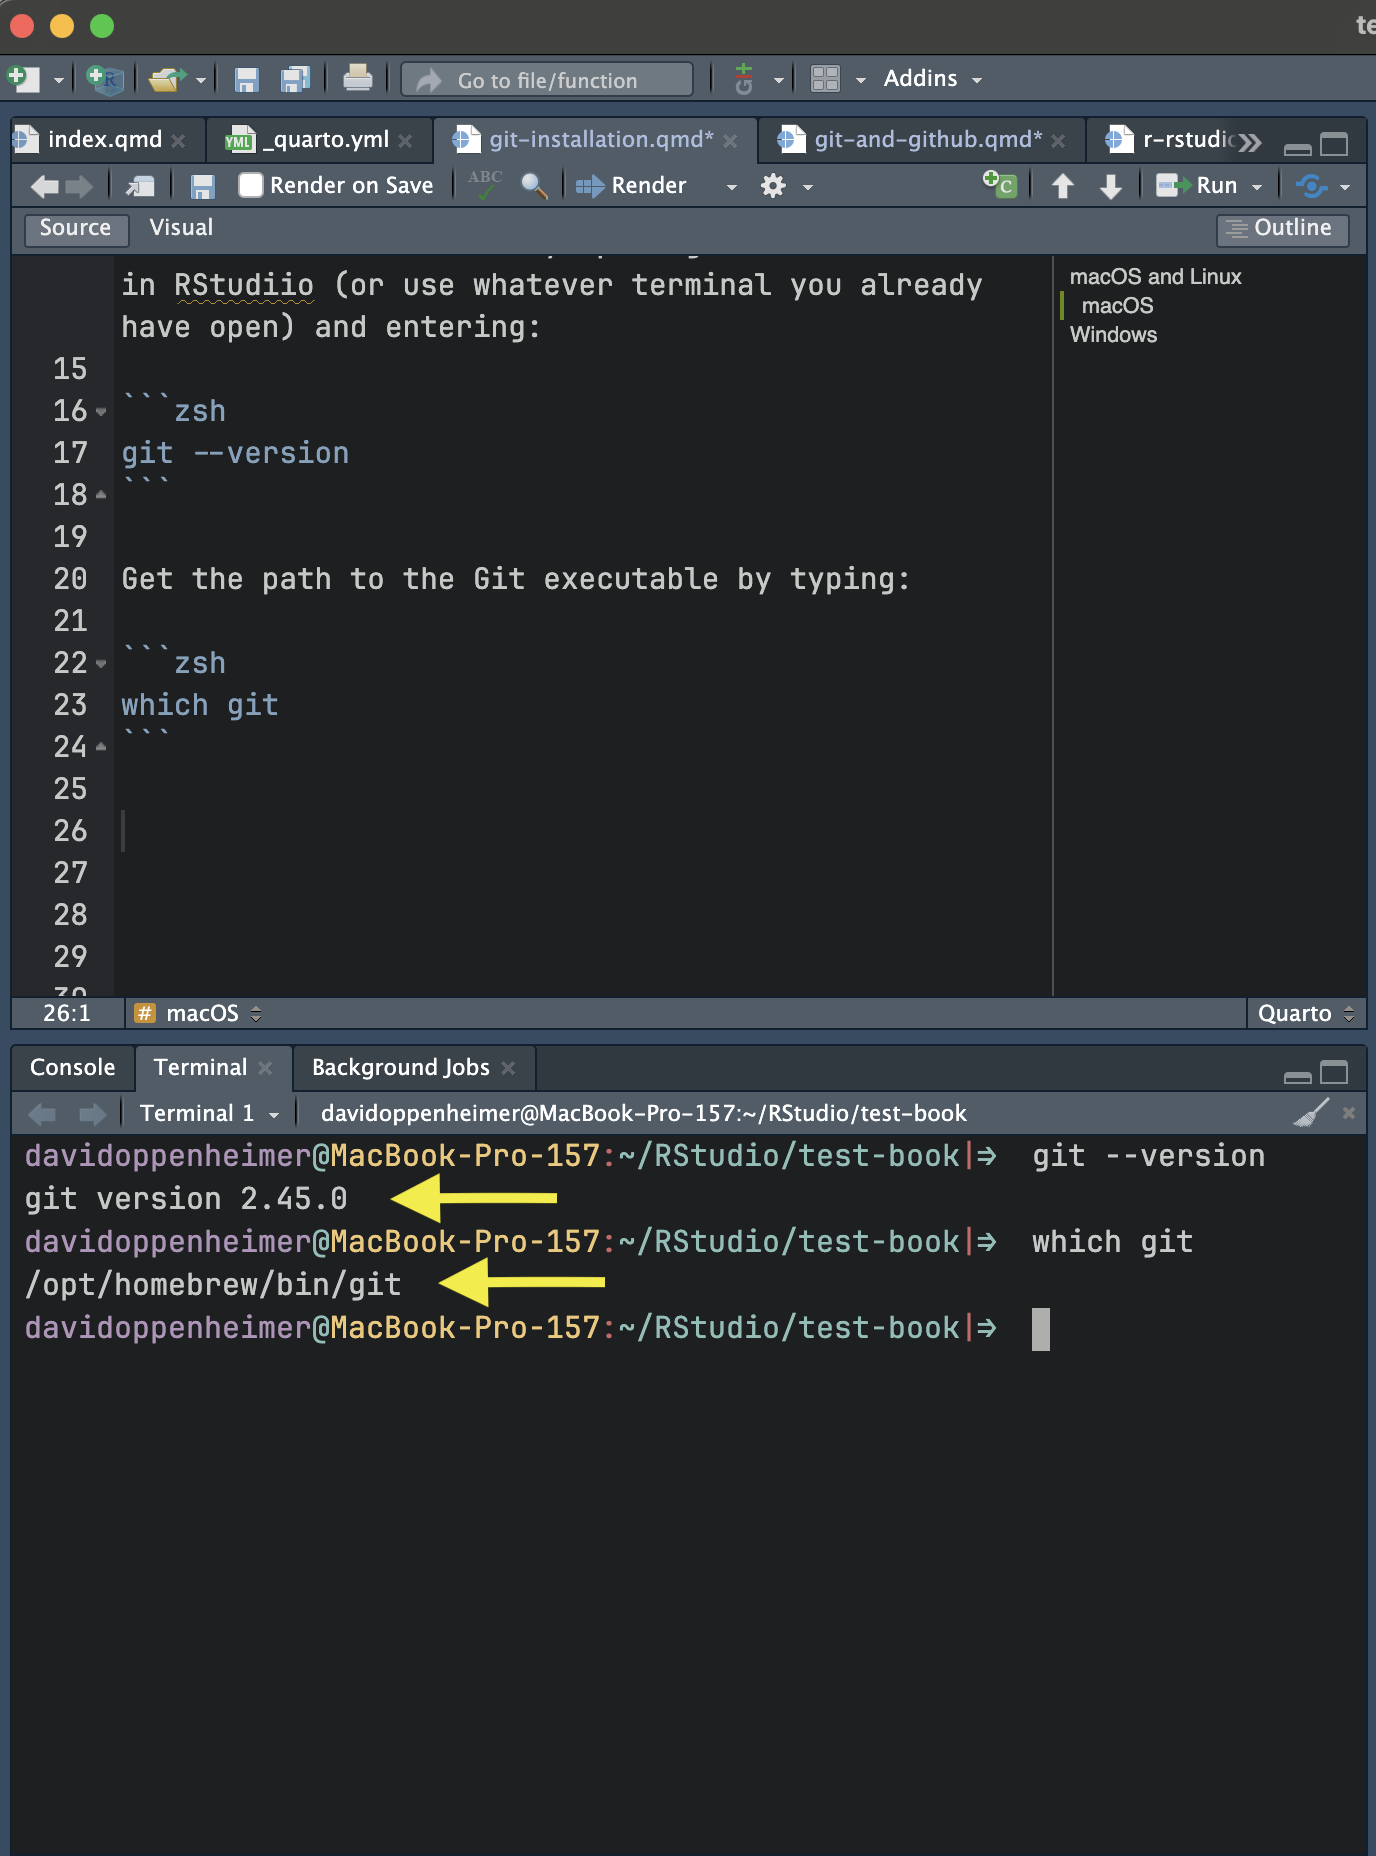
\includegraphics[width=0.6\textwidth,height=\textheight]{../assets/git-version.png}

}

\caption{RStudio Terminal window}

\end{figure}%

Next, in RStudio, go to \emph{Tools} → \emph{Global Options}. You will
get the menu in \emph{(a)}:

\begin{figure}

\begin{minipage}{0.50\linewidth}

\centering{

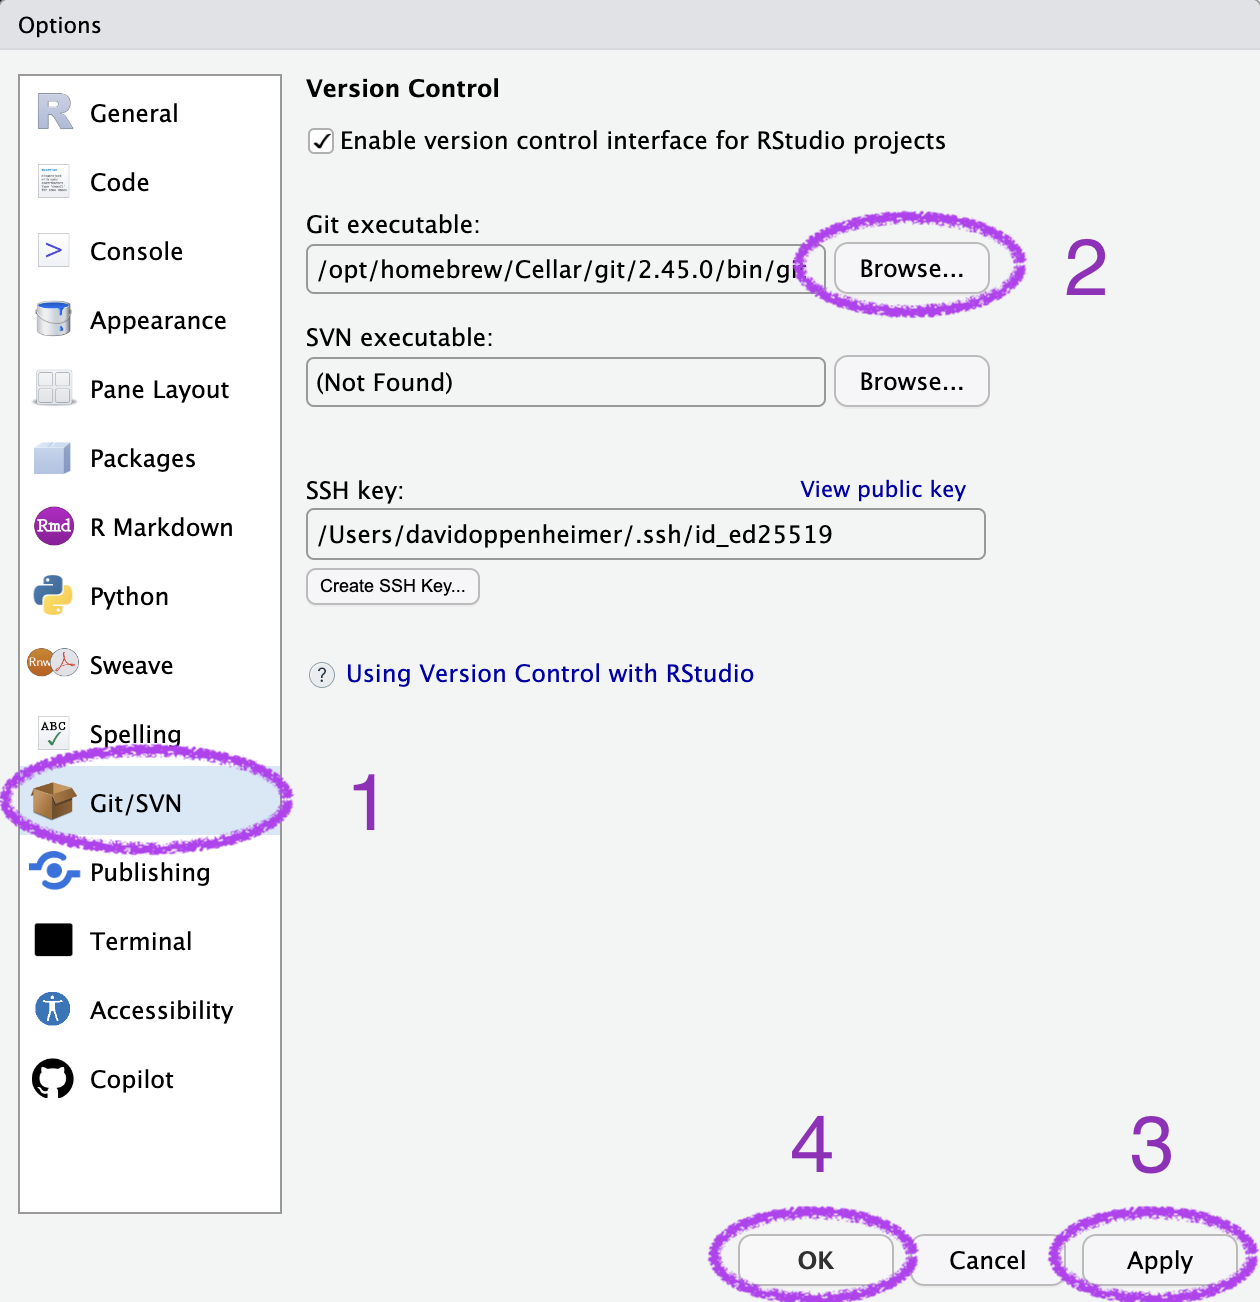
\includegraphics{../assets/git-path.png}

}

\subcaption{\label{fig-options}Global Options}

\end{minipage}%
%
\begin{minipage}{0.50\linewidth}

\centering{

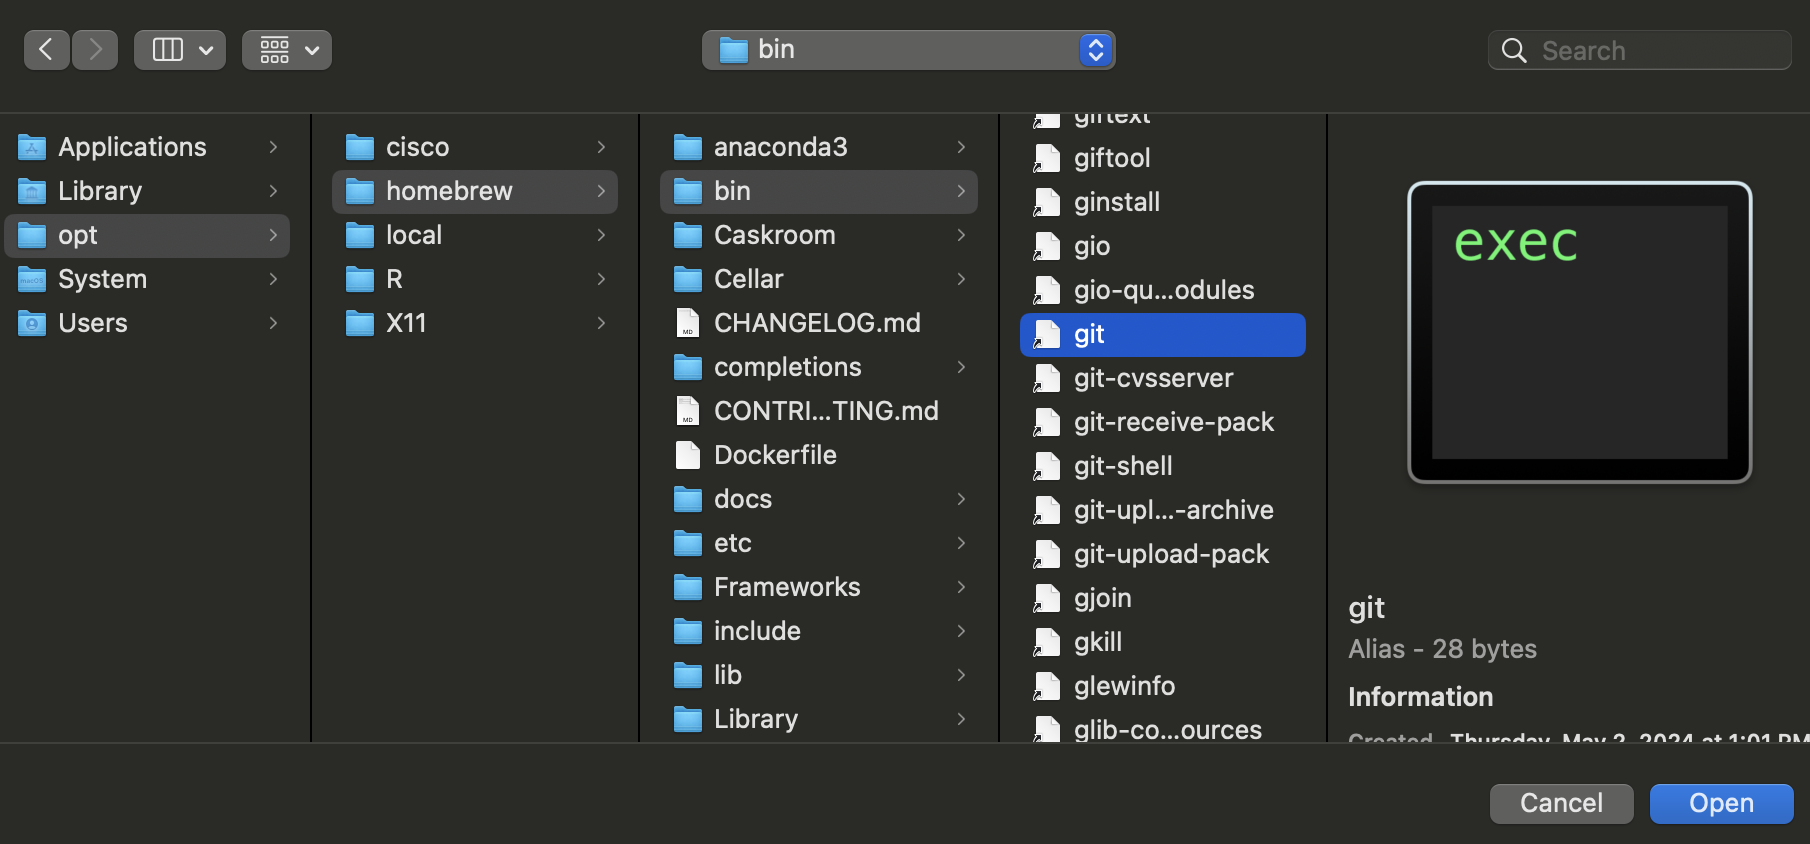
\includegraphics{../assets/git-path-browse.png}

}

\subcaption{\label{fig-path}git path}

\end{minipage}%

\caption{\label{fig-git}Setting the Git path in RStudio}

\end{figure}%

\begin{enumerate}
\def\labelenumi{\arabic{enumi}.}
\tightlist
\item
  Choose \emph{Git/SVN}.
\item
  Browse to \texttt{git} using the path obtained from the
  \texttt{which\ git} command. See \emph{(b)}, above.
\item
  Click \emph{Apply}.
\item
  Click \emph{OK}.
\end{enumerate}

\begin{tcolorbox}[enhanced jigsaw, left=2mm, title=\textcolor{quarto-callout-note-color}{\faInfo}\hspace{0.5em}{Note}, opacityback=0, breakable, colbacktitle=quarto-callout-note-color!10!white, colframe=quarto-callout-note-color-frame, arc=.35mm, titlerule=0mm, leftrule=.75mm, opacitybacktitle=0.6, toptitle=1mm, colback=white, toprule=.15mm, bottomtitle=1mm, rightrule=.15mm, coltitle=black, bottomrule=.15mm]

The \texttt{git} executable in \texttt{/opt/homebrew/bin/git} is an
alias that points to \texttt{/opt/homebrew/Cellar/git/2.45.0/bin/git}.
When you browse to \texttt{/opt/homebrew/bin/git}, it gets resolved to
the correct path.

\end{tcolorbox}

Now RStudio will use the updated Git.

\subsection{Windows}\label{windows}

Windows users should go to the \href{https://git-scm.com/}{Git website}
to get the latest Windows build.

\section{Get a GitHub Account}\label{get-a-github-account}

\subsection{Linking RStudio to GitHub}\label{linking-rstudio-to-github}

\subsubsection{ssh keys}\label{ssh-keys}

See \href{https://happygitwithr.com/ssh-keys}{Chapter 10 Set up keys for
SSH}. I already have a key pair that I have used for GitHub.

\begin{enumerate}
\def\labelenumi{\arabic{enumi}.}
\item
  Add key to \texttt{ssh-agent}. Use the following command in the
  terminal:

\begin{Shaded}
\begin{Highlighting}[]
\BuiltInTok{eval} \StringTok{"}\VariableTok{$(}\FunctionTok{ssh{-}agent} \AttributeTok{{-}s}\VariableTok{)}\StringTok{"}
\end{Highlighting}
\end{Shaded}

  You should see a response like the following, except the \texttt{pid}
  number will likely be different.

\begin{Shaded}
\begin{Highlighting}[]
\ExtensionTok{Agent}\NormalTok{ pid 15360}
\end{Highlighting}
\end{Shaded}
\item
  If you use MacOS \textgreater{} 10.12.1, create a file
  \texttt{\textasciitilde{}/.ssh/config} with the following contents:

\begin{Shaded}
\begin{Highlighting}[]
\ExtensionTok{Host} \PreprocessorTok{*}
\ExtensionTok{AddKeysToAgent}\NormalTok{ yes}
\ExtensionTok{UseKeychain}\NormalTok{ yes}
\ExtensionTok{IdentityFile}\NormalTok{ \textasciitilde{}/.ssh/id\_ed25519}
\end{Highlighting}
\end{Shaded}
\item
  Add your key to the \texttt{ssh-agent}.

\begin{Shaded}
\begin{Highlighting}[]
\FunctionTok{ssh{-}add} \AttributeTok{{-}{-}apple{-}load{-}keychain}\NormalTok{ \textasciitilde{}/.ssh/id\_ed25519}
\end{Highlighting}
\end{Shaded}

  You should now be able to push to GitHub!
\end{enumerate}

If you are asked for a username and password after setting ssh keys, try
the following:

\begin{Shaded}
\begin{Highlighting}[]
\FunctionTok{git}\NormalTok{ remote }\AttributeTok{{-}v}
\ExtensionTok{origin}\NormalTok{  https://github.com/dgoppenheimer/notebook{-}template.git }\ErrorTok{(}\ExtensionTok{fetch}\KeywordTok{)}
\ExtensionTok{origin}\NormalTok{  https://github.com/dgoppenheimer/notebook{-}template.git }\ErrorTok{(}\ExtensionTok{push}\KeywordTok{)}
\end{Highlighting}
\end{Shaded}

If you get the \texttt{https://...} response from git, then you need to
change how you access the remote repository.

\begin{Shaded}
\begin{Highlighting}[]
\FunctionTok{git}\NormalTok{ remote set{-}url origin git@github.com:dgoppenheimer/notebook{-}template.git}
\end{Highlighting}
\end{Shaded}

Now, you should be able to push without needed to enter a
username/password.

\section{Get the Notebook}\label{get-the-notebook}

\begin{enumerate}
\def\labelenumi{\arabic{enumi}.}
\item
  Ask to be a collaborator on the \texttt{notebook-template} repository.
\item
  Click the \emph{notifications} icon on GitHub.

  \begin{center}
  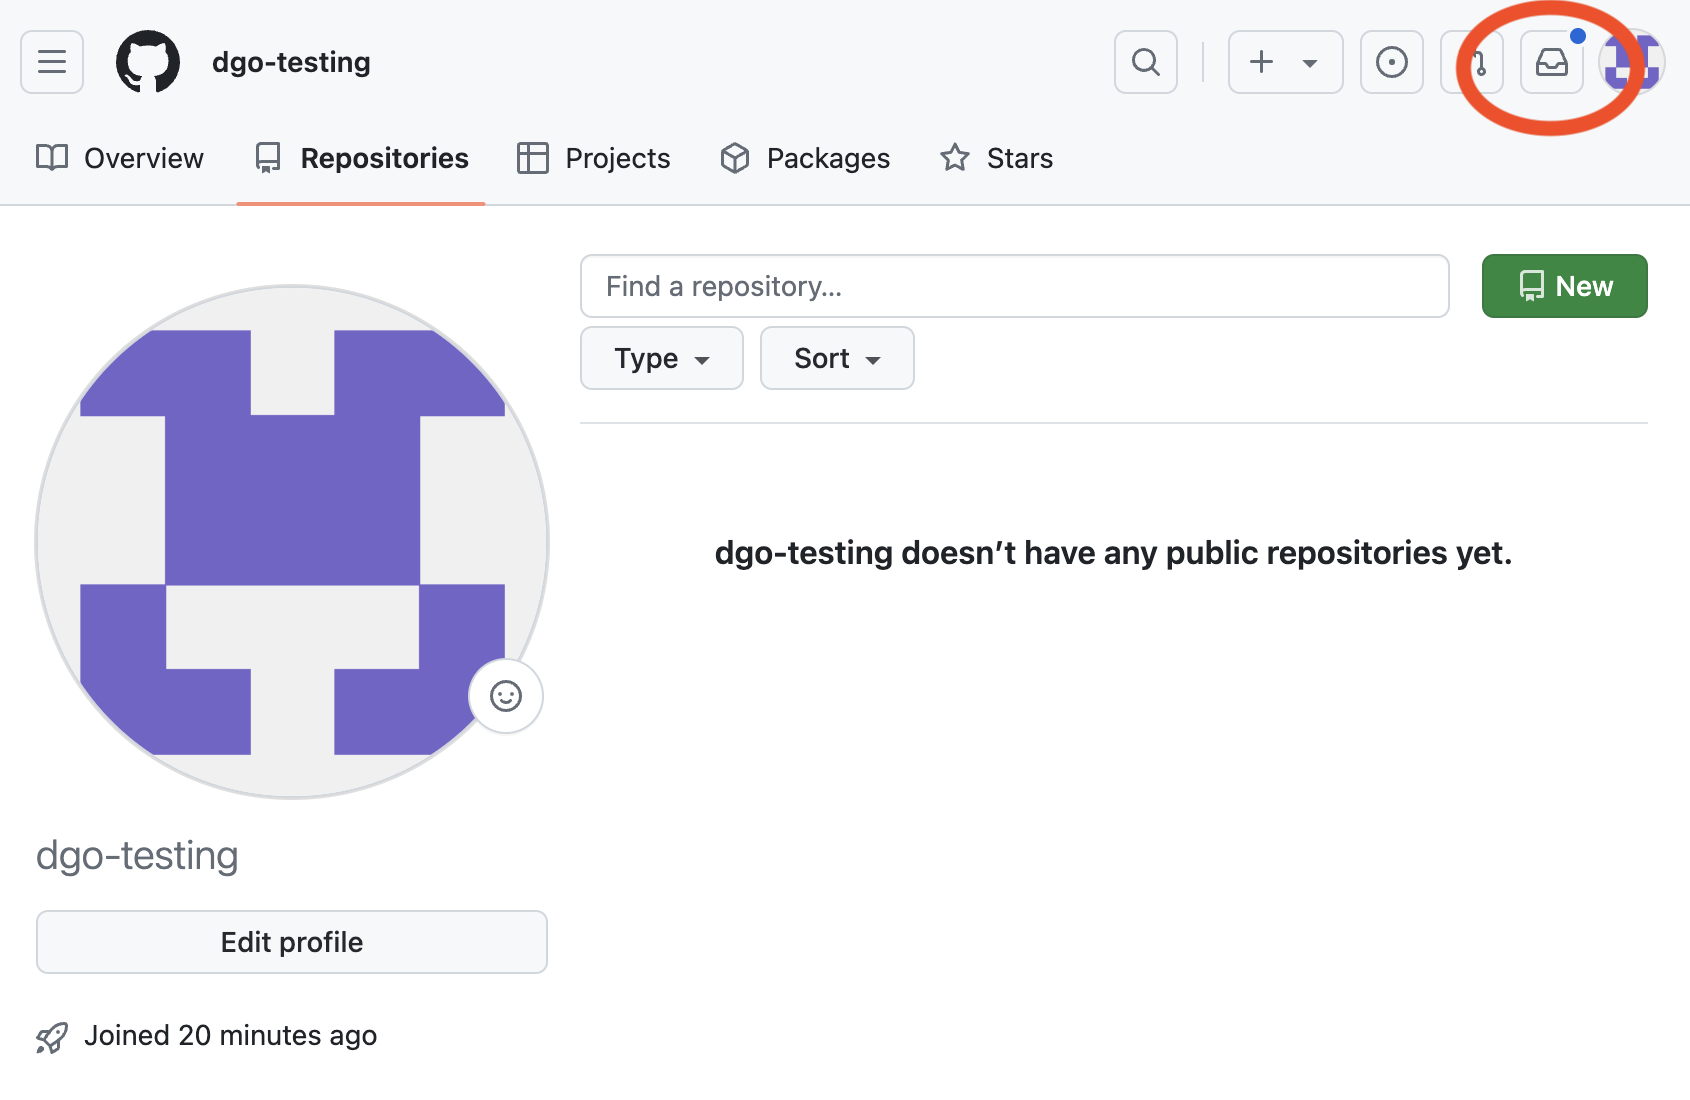
\includegraphics[width=0.75\textwidth,height=\textheight]{../assets/github-notification1.png}
  \end{center}
\item
  On the notifications page, click the \emph{invitation to join
  \ldots{}} row.

  \begin{center}
  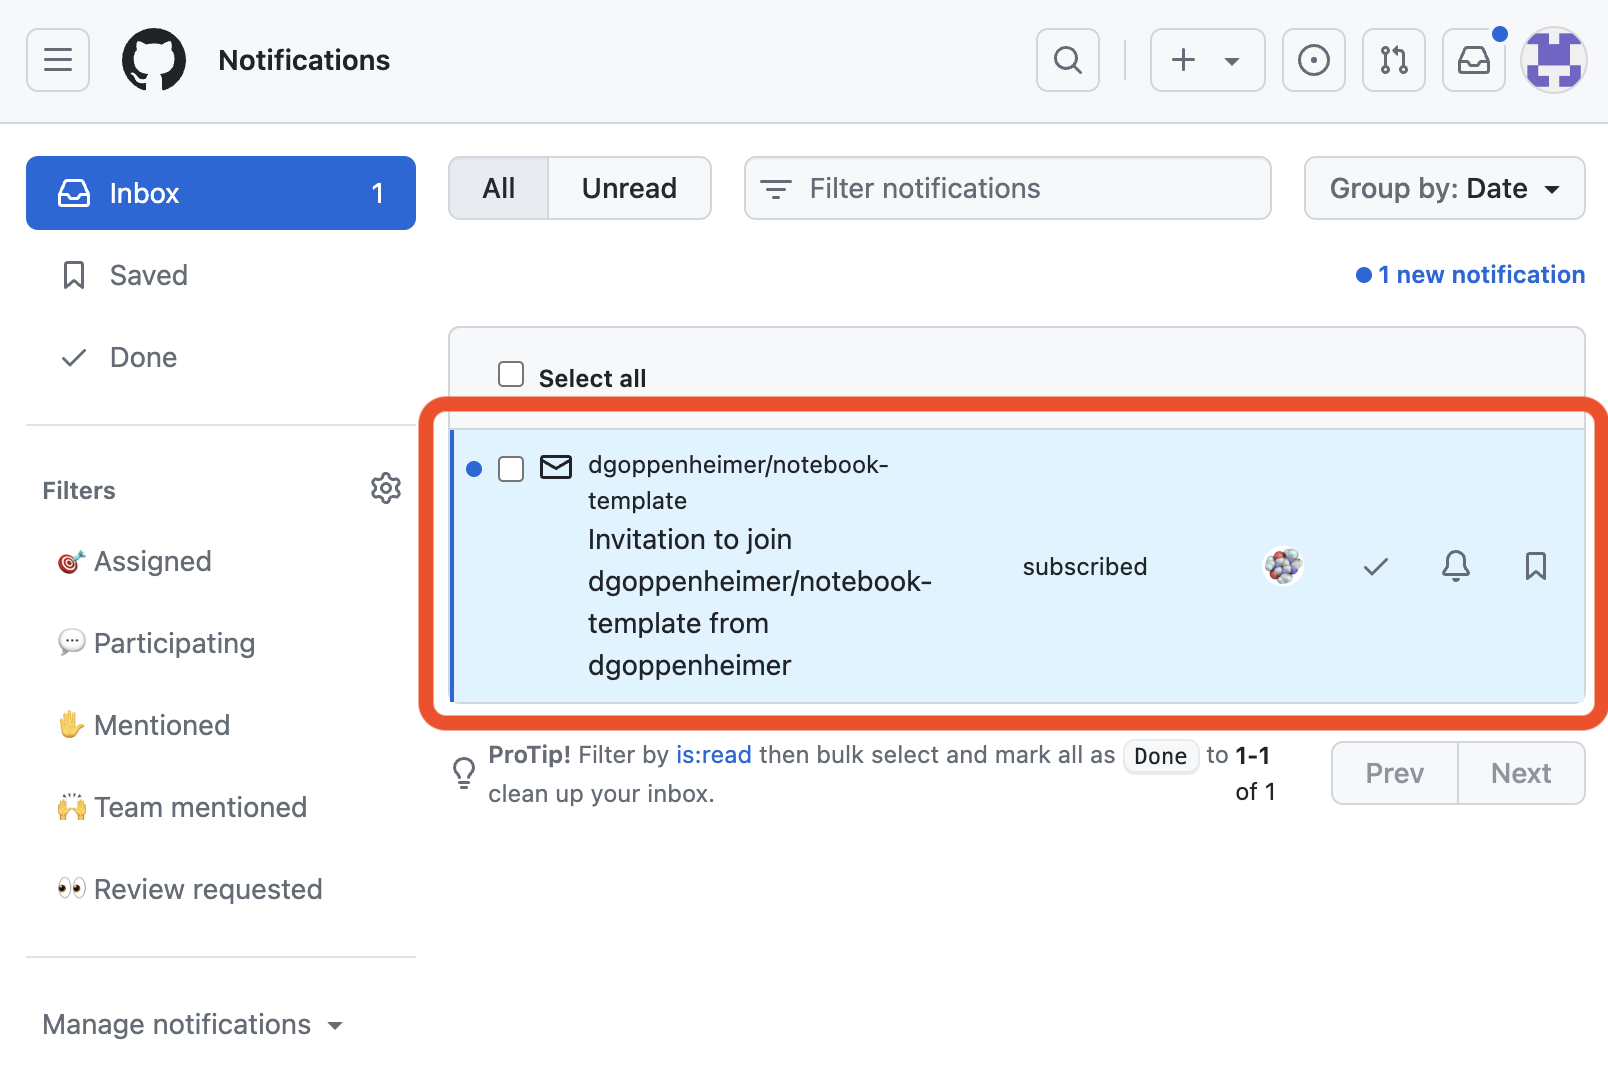
\includegraphics[width=0.75\textwidth,height=\textheight]{../assets/github-colab.png}
  \end{center}
\item
  Click the \emph{Accept} button to accept the invitation.

  \begin{center}
  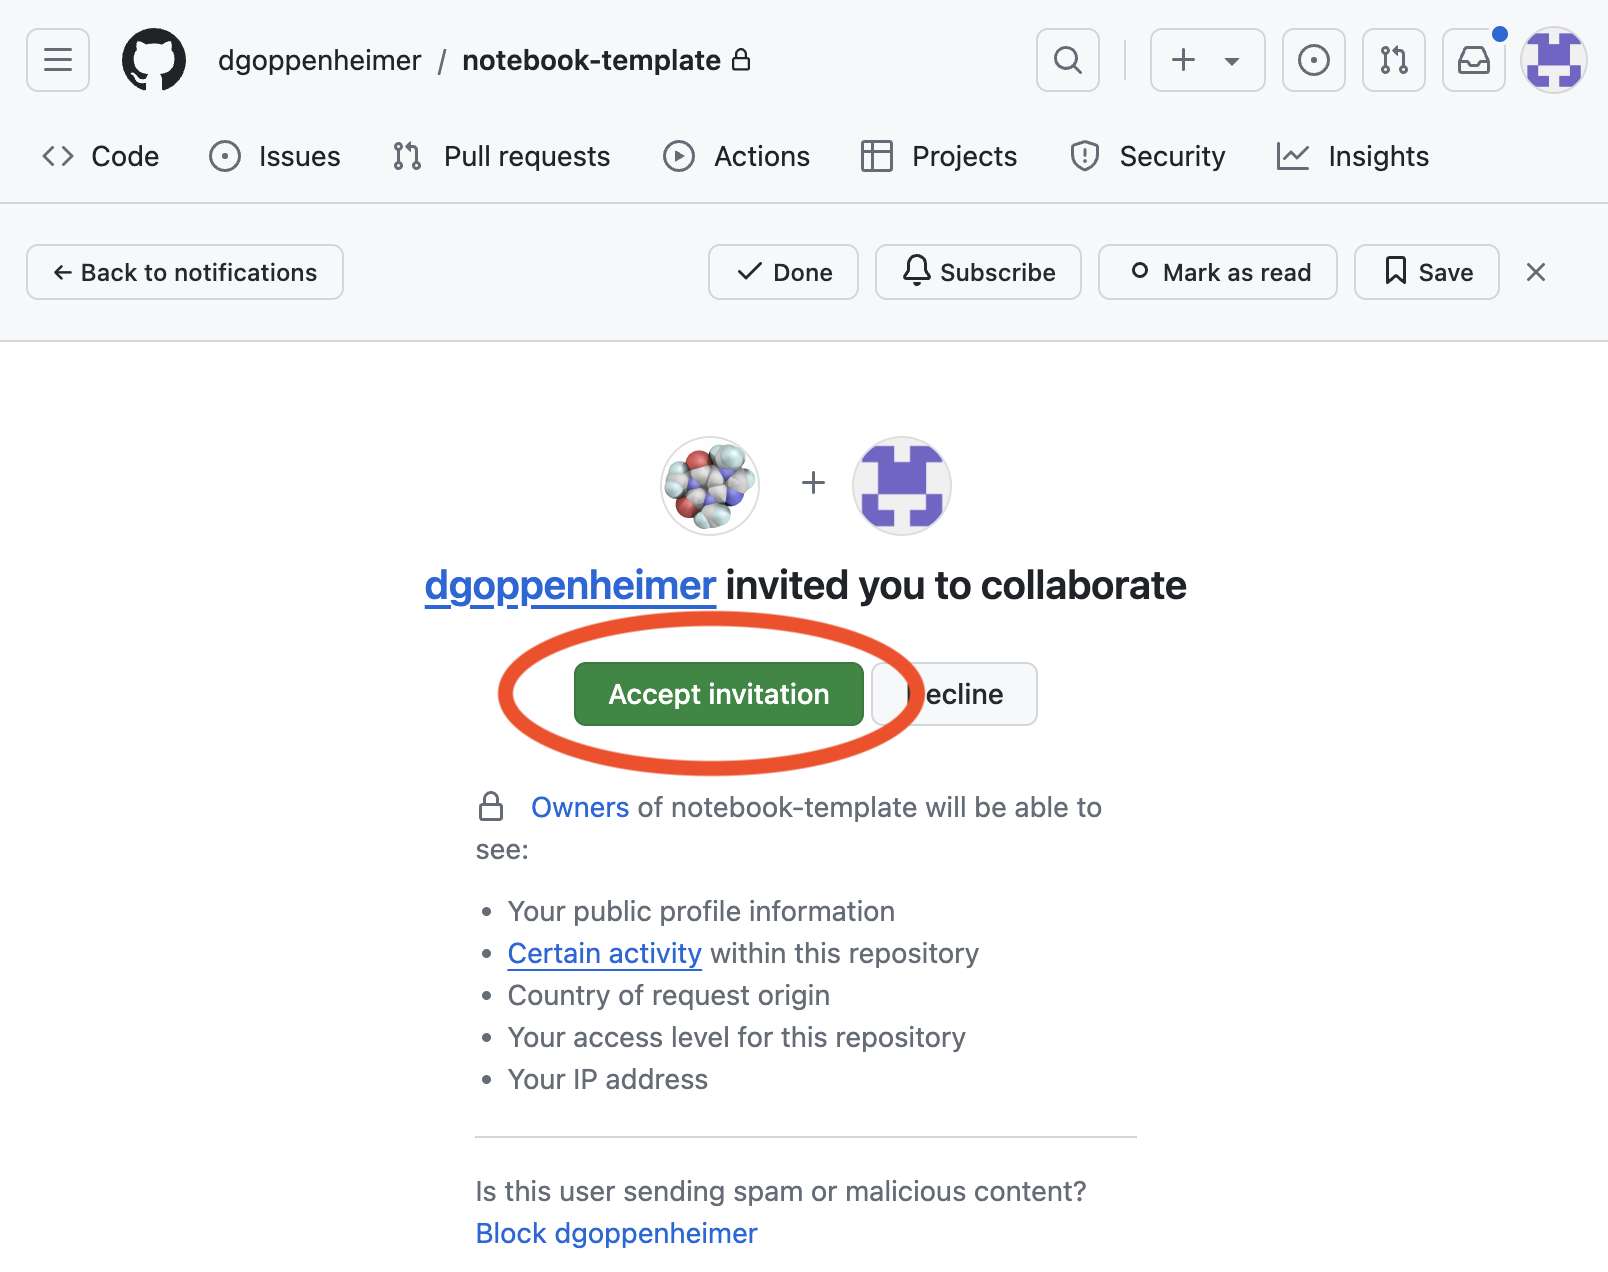
\includegraphics[width=0.75\textwidth,height=\textheight]{../assets/github-accept.png}
  \end{center}
\item
  Click the \emph{Fork} button to create your own fork of this project.

  \begin{center}
  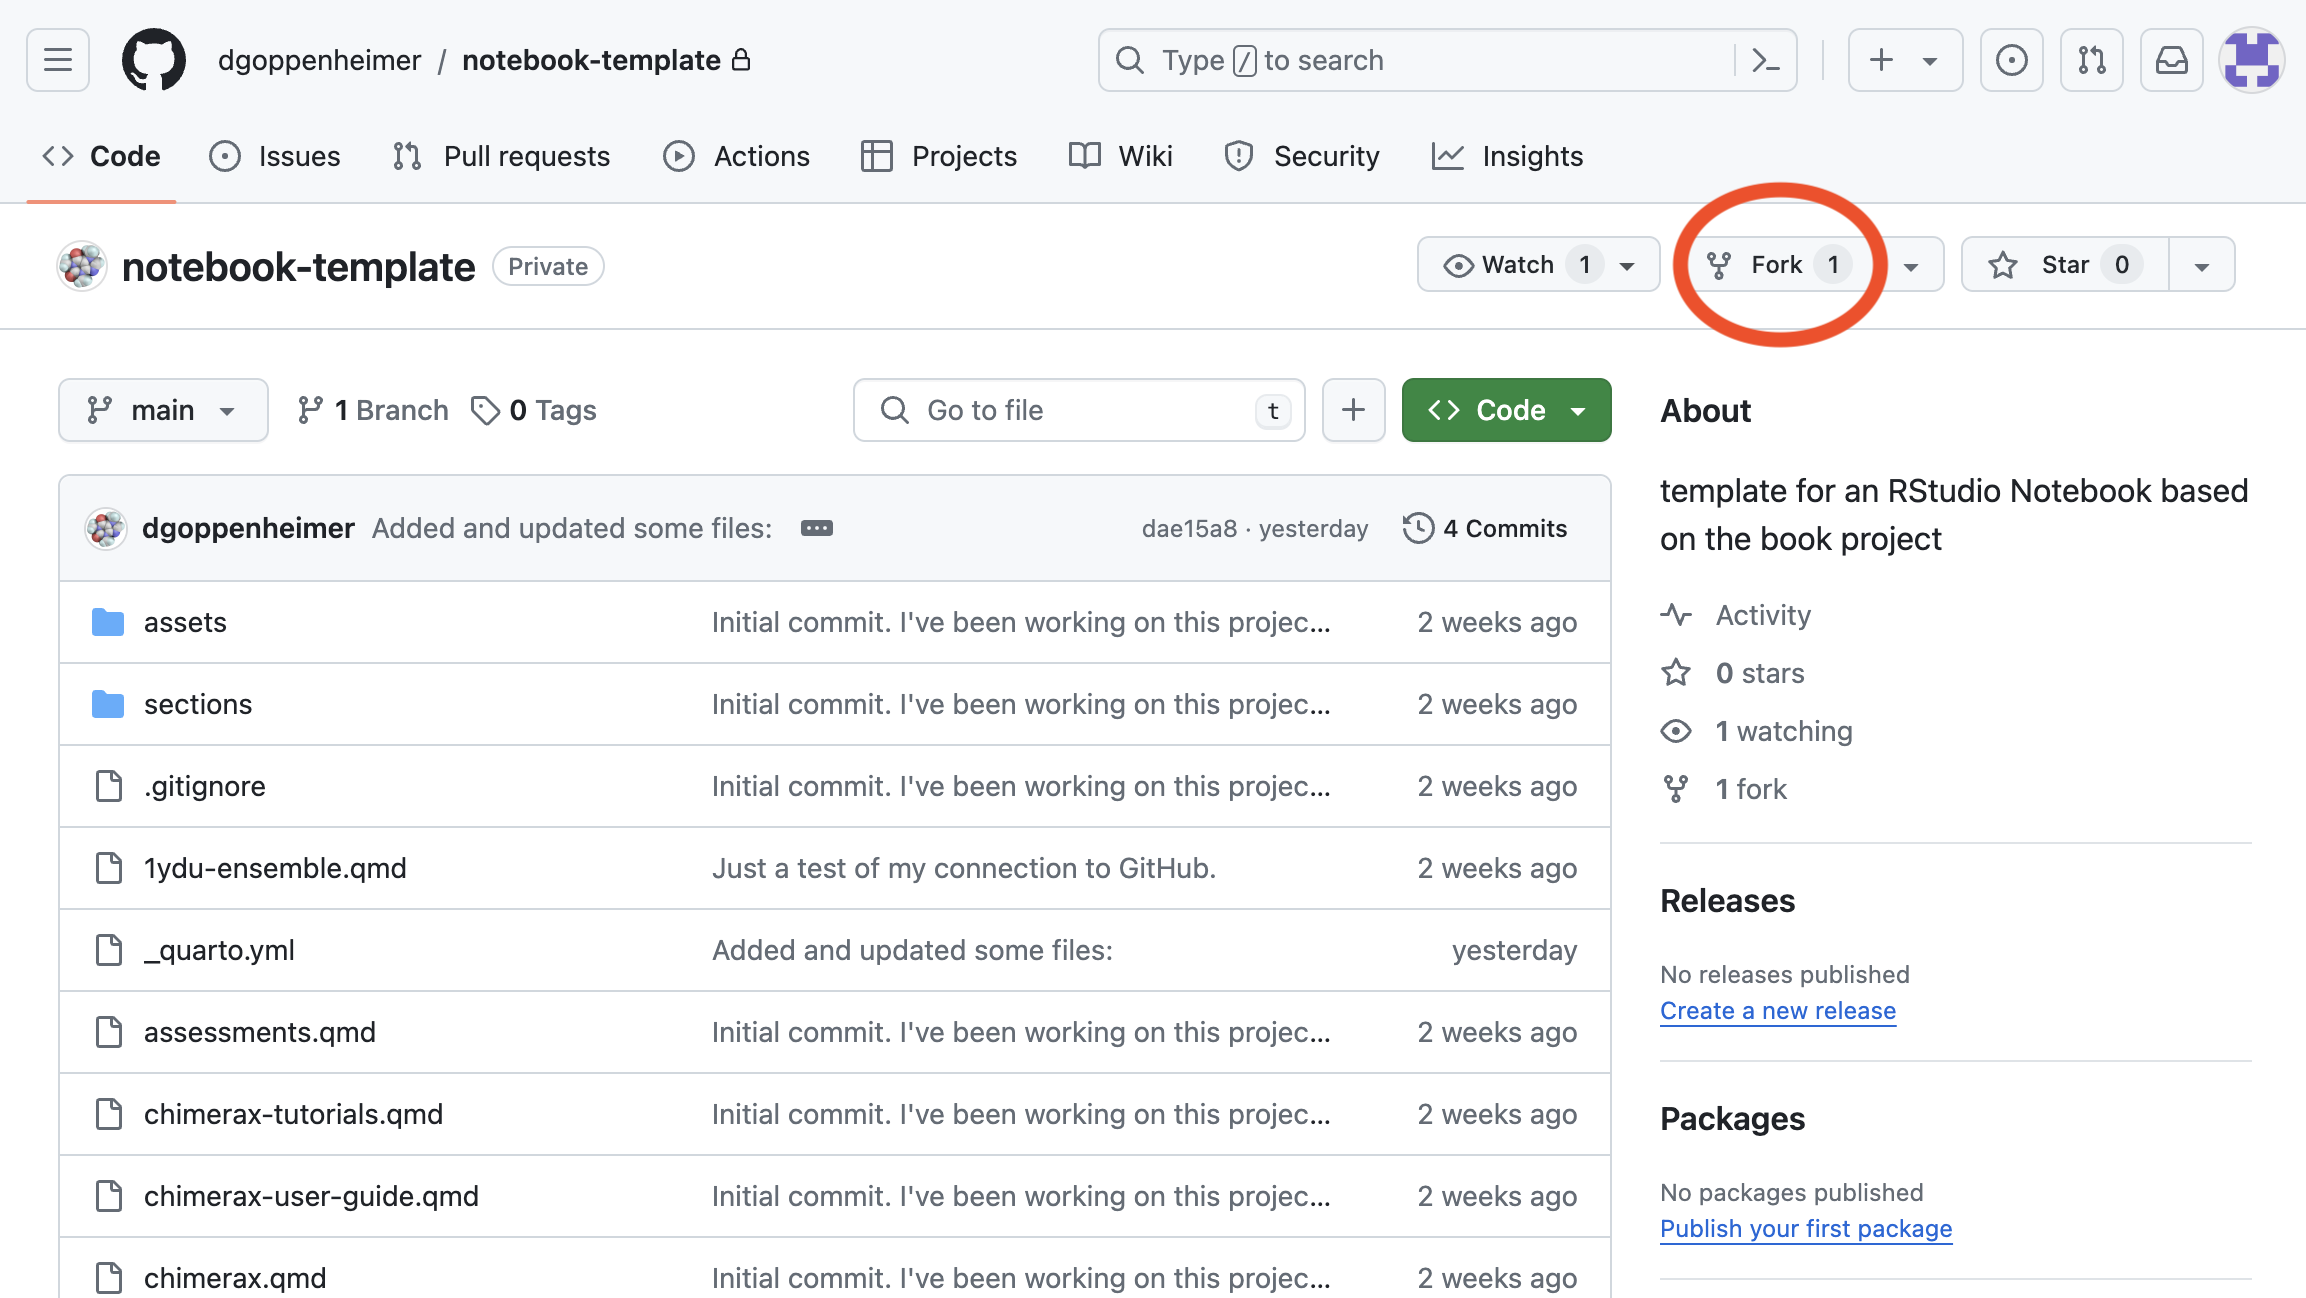
\includegraphics[width=0.75\textwidth,height=\textheight]{../assets/github-fork.png}
  \end{center}
\item
  Give the project a new name. Use a name that describes the project
  (Hif1alpha, p53TAD, etc.). Here I chose \texttt{test-fork-notebook}
  because I am using this fork for testing purposes. Then click
  \emph{Create fork}.

  \begin{center}
  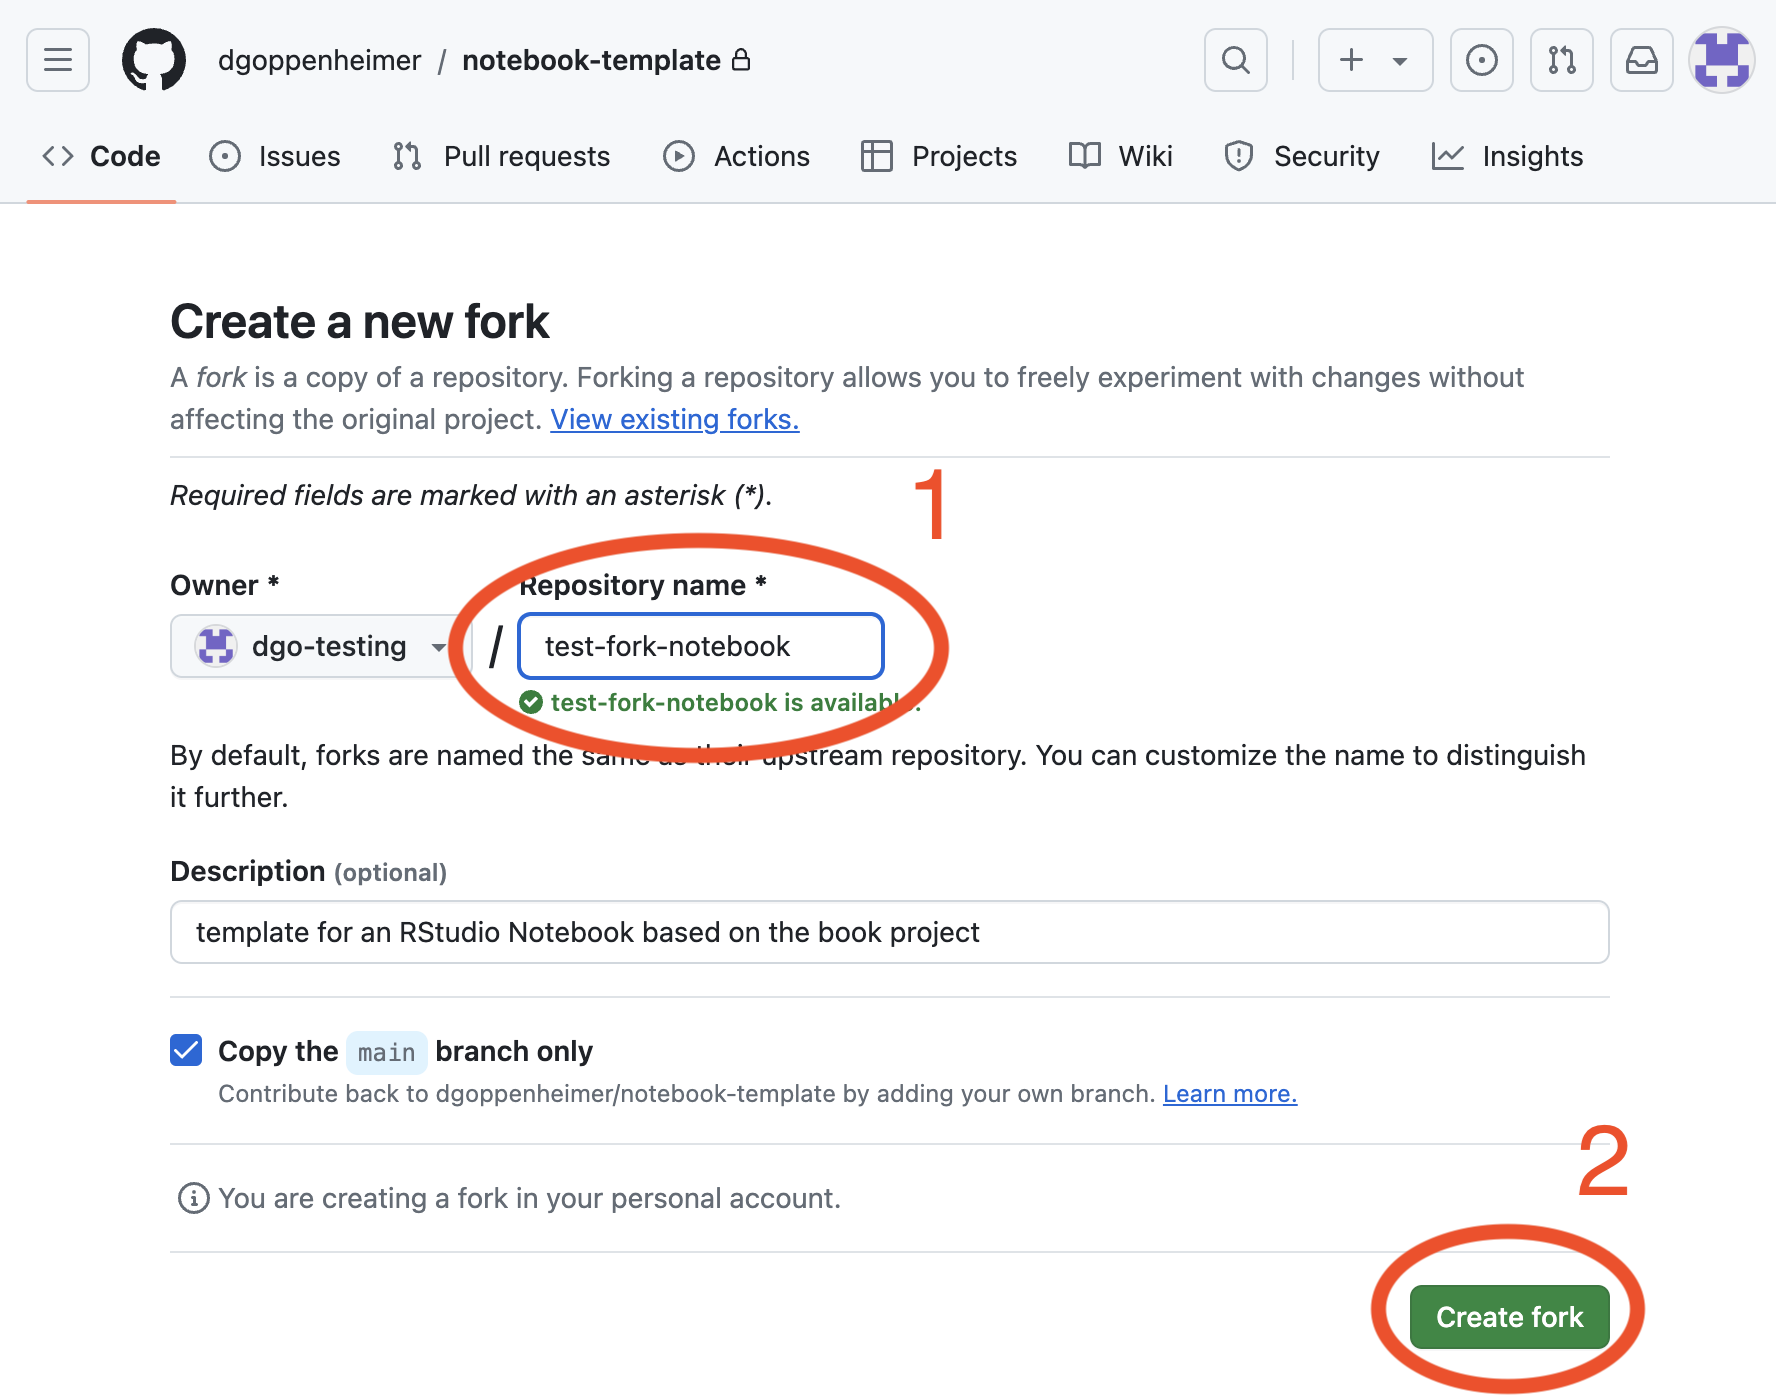
\includegraphics[width=0.75\textwidth,height=\textheight]{../assets/github-fork-name.png}
  \end{center}

  Now you have your own copy of the Notebook template.
\item
  Clone the forked repository. On your local computer, Create a new
  project in RStudio. The \emph{New Project Wizard} will open. Choose
  the \emph{Version Control} option.

  \begin{center}
  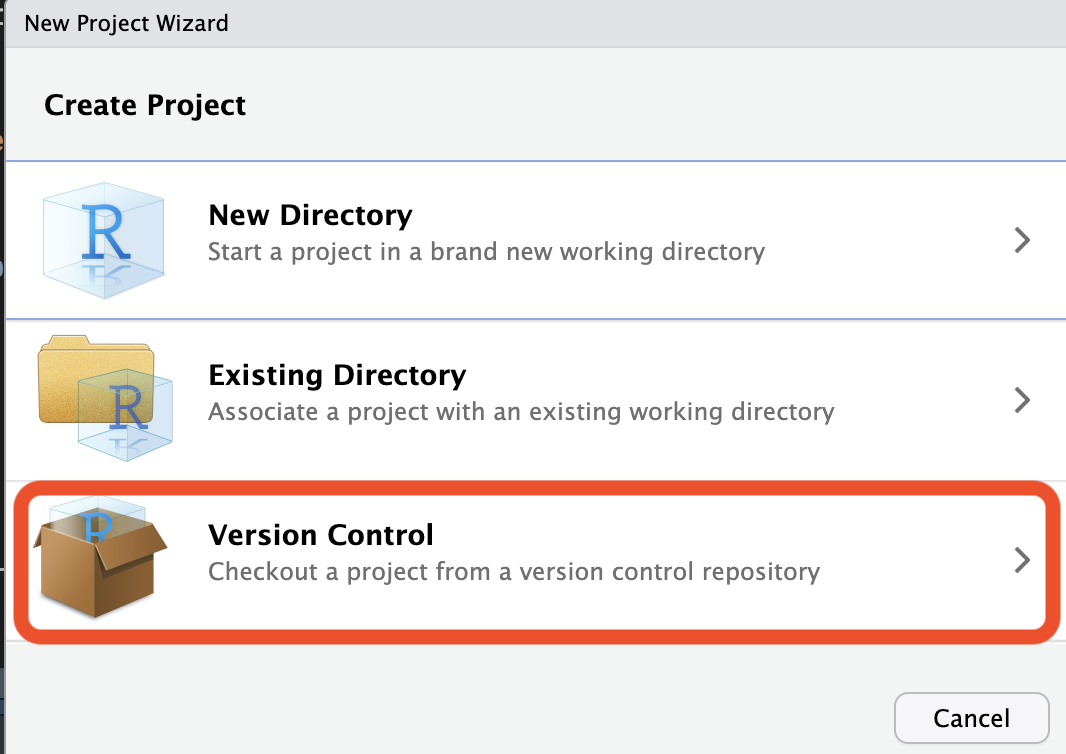
\includegraphics[width=0.75\textwidth,height=\textheight]{../assets/rstudio-new-project.png}
  \end{center}
\item
  Choose the \emph{Git} option.

  \begin{center}
  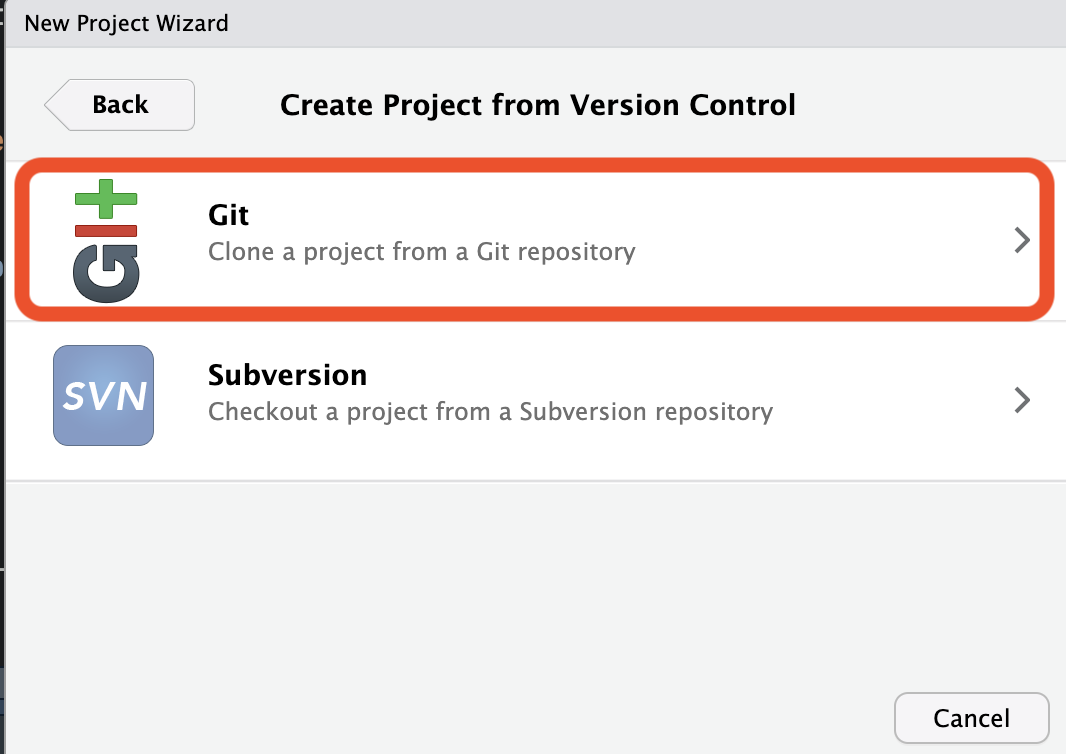
\includegraphics[width=0.75\textwidth,height=\textheight]{../assets/rstudio-git-project.png}
  \end{center}
\item
  Go to your repository page on GitHub in your browser.

  \begin{enumerate}
  \def\labelenumii{\arabic{enumii}.}
  \tightlist
  \item
    Click the \emph{Code} button.
  \item
    Choose \emph{HTTPS}.
  \item
    Copy the URL to your clipboard.
  \end{enumerate}

  \begin{center}
  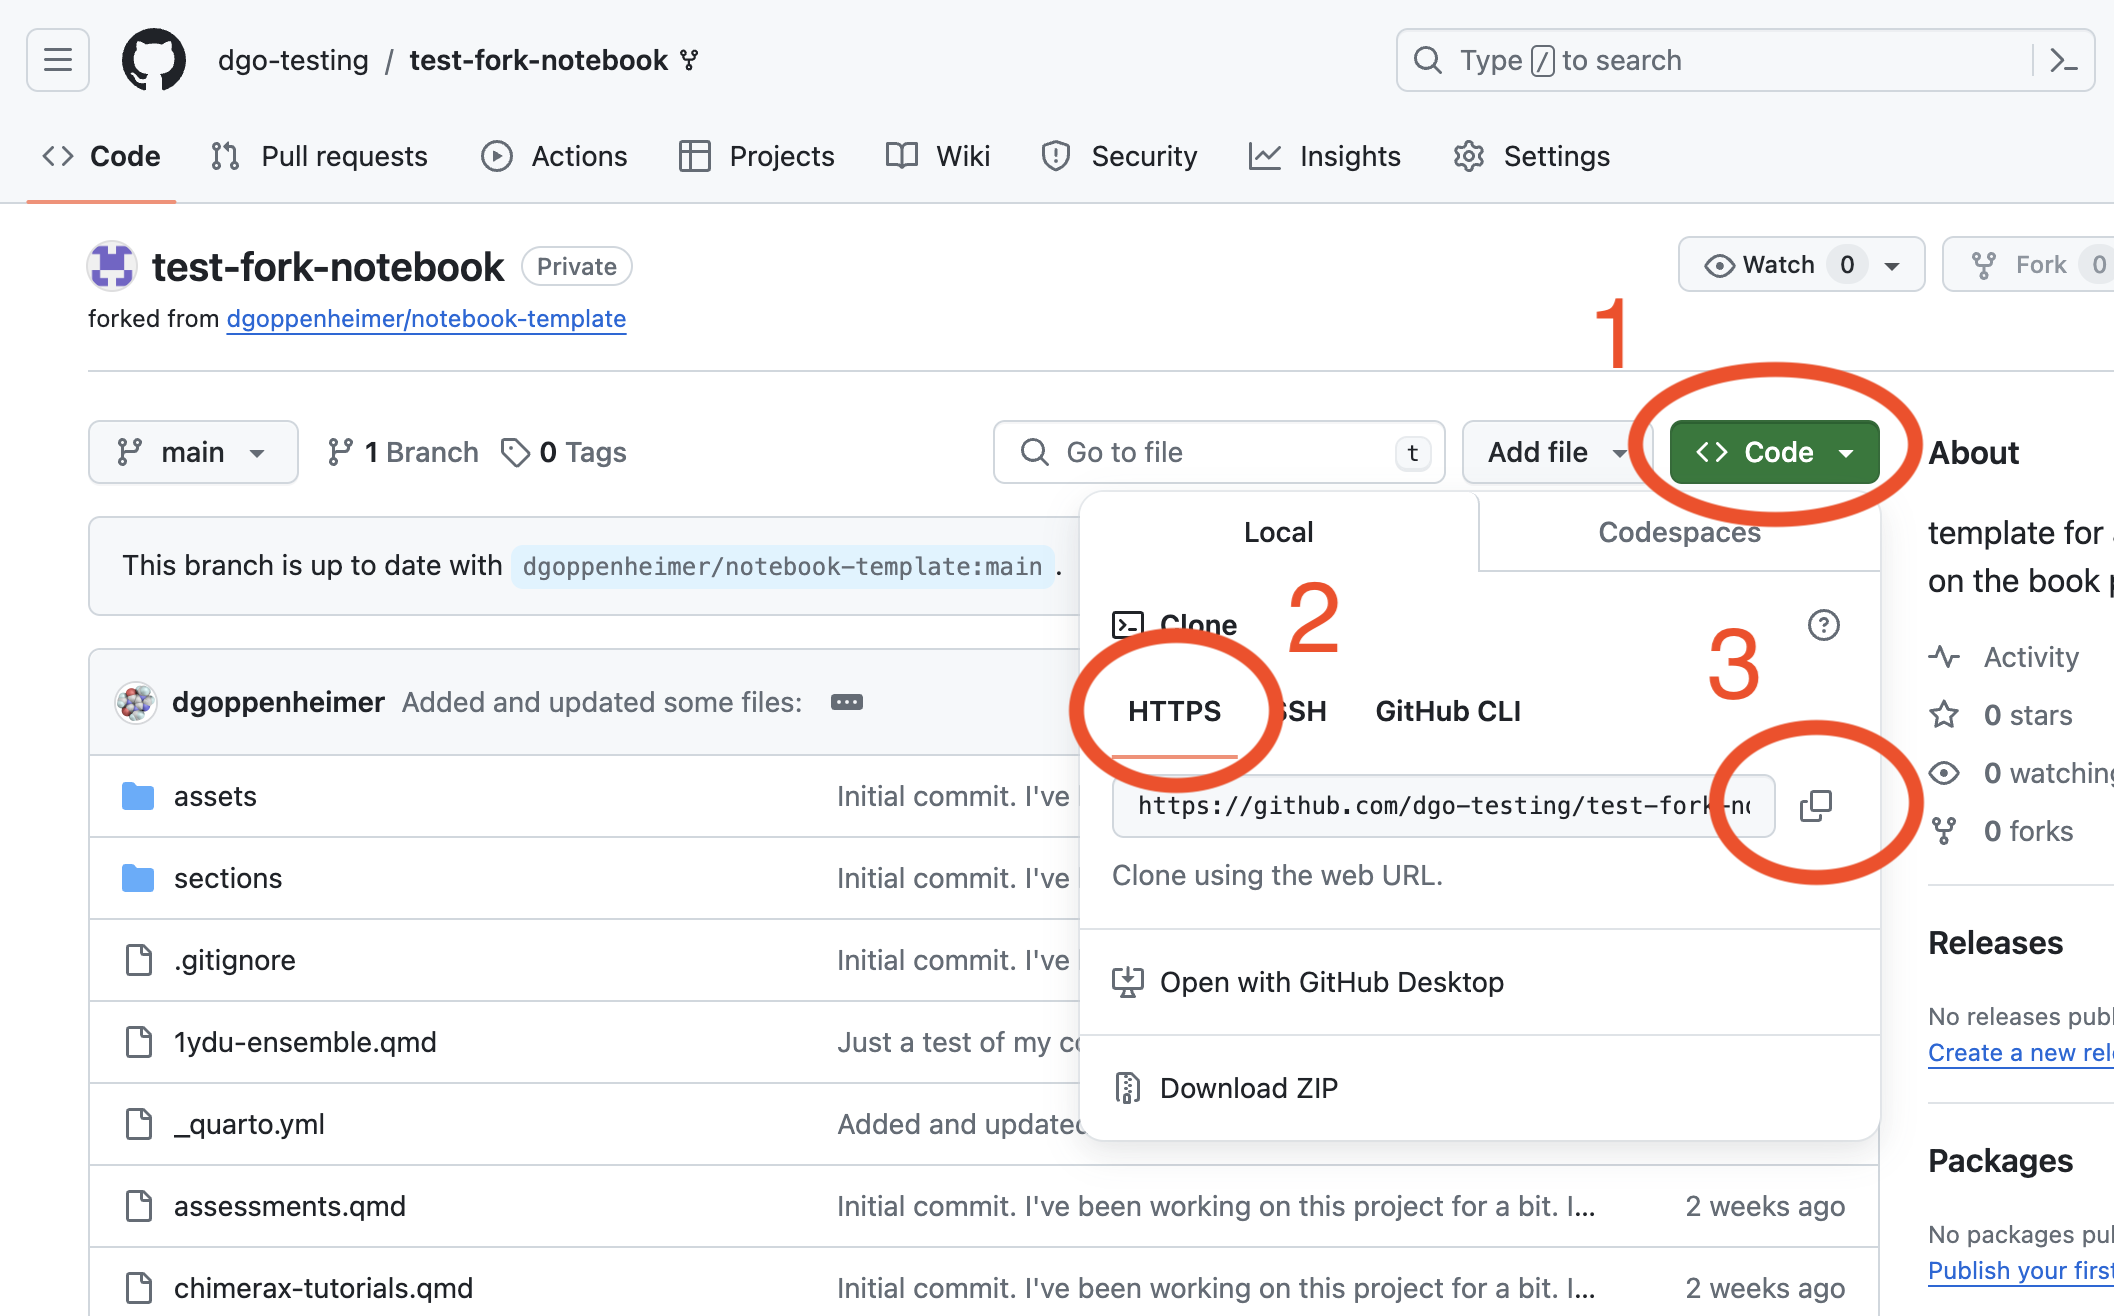
\includegraphics[width=0.75\textwidth,height=\textheight]{../assets/github-project-url.png}
  \end{center}
\item
  Go back to the \emph{RStudio New Project Wizard} window.

  \begin{enumerate}
  \def\labelenumii{\arabic{enumii}.}
  \tightlist
  \item
    Paste in the URL that you copied from your GitHub project page.
  \item
    Choose a name for the directory for the project. I usually make the
    directory name the same as the GitHub project name, in this case,
    \texttt{test-fork-notebook}.
  \item
    Click \emph{Create Project}. The project will be cloned into the
    directory that you specified.
  \end{enumerate}

  \begin{center}
  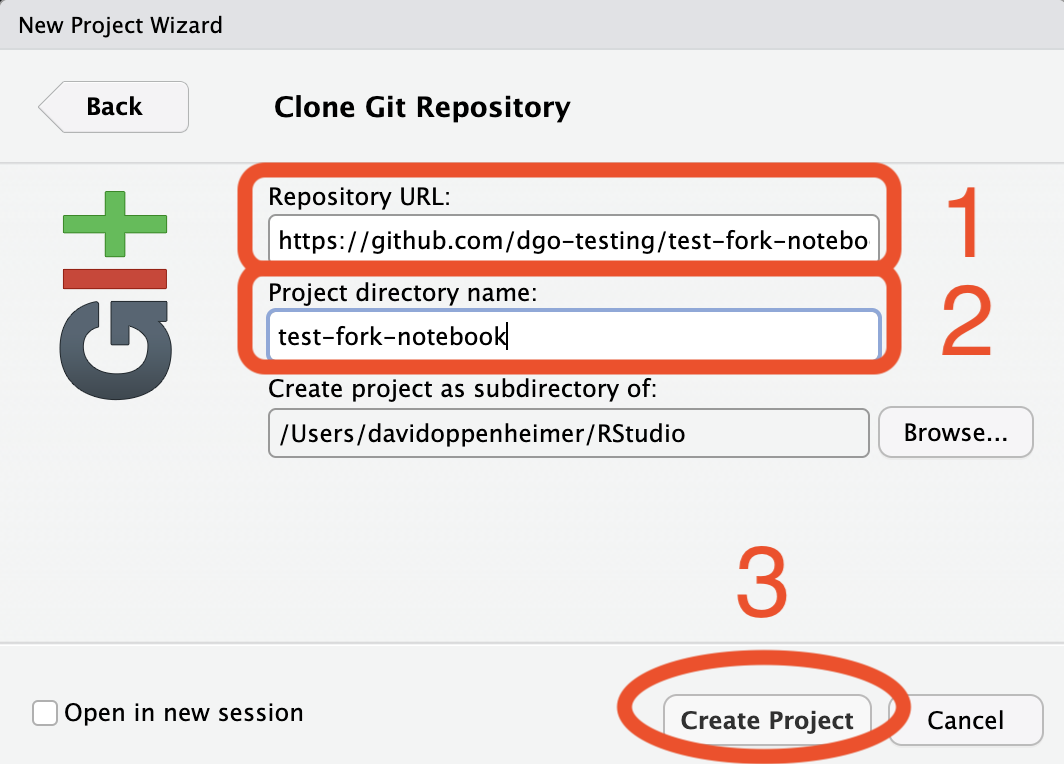
\includegraphics[width=0.75\textwidth,height=\textheight]{../assets/rstudio-git-project2.png}
  \end{center}

  You now have your new project in your local directory linked to the
  repository in GitHub. Make changes/additions, do \texttt{git\ add\ .},
  \texttt{git\ commit\ -m\ "added\ new\ files"}, and \texttt{git\ push},
  to push the changes to GitHub.
\end{enumerate}

\section{Keeping the forked Notebook in sync with the original
project}\label{keeping-the-forked-notebook-in-sync-with-the-original-project}

Hopefully you will not need to do this often, but the steps below will
import any changes to the original project while keeping all the changes
you have made to the forked project.

\subsection{\texorpdfstring{Define the \texttt{upstream}
repository}{Define the upstream repository}}\label{define-the-upstream-repository}

From
\href{https://docs.github.com/en/pull-requests/collaborating-with-pull-requests/working-with-forks/configuring-a-remote-repository-for-a-fork}{GitHub
Docs Configuring a remote repository for a fork}.

\begin{enumerate}
\def\labelenumi{\arabic{enumi}.}
\item
  Open Terminal.
\item
  List the current configured remote repository for your fork.

\begin{Shaded}
\begin{Highlighting}[]
\ExtensionTok{$}\NormalTok{ git remote }\AttributeTok{{-}v}
\OperatorTok{\textgreater{}}\NormalTok{ origin  }\ExtensionTok{https://github.com/YOUR{-}USERNAME/YOUR{-}FORK.git} \ErrorTok{(}\ExtensionTok{fetch}\KeywordTok{)}
\OperatorTok{\textgreater{}}\NormalTok{ origin  }\ExtensionTok{https://github.com/YOUR{-}USERNAME/YOUR{-}FORK.git} \ErrorTok{(}\ExtensionTok{push}\KeywordTok{)}
\end{Highlighting}
\end{Shaded}
\item
  Specify a new remote \texttt{upstream} repository that will be synced
  with the fork. This is the original repository that we created our
  fork from.

\begin{Shaded}
\begin{Highlighting}[]
\FunctionTok{git}\NormalTok{ remote add upstream https://github.com/dgoppenheimer/notebook{-}template.git}
\end{Highlighting}
\end{Shaded}
\item
  Verify the new upstream repository you've specified for your fork.

\begin{Shaded}
\begin{Highlighting}[]
\FunctionTok{git}\NormalTok{ remote }\AttributeTok{{-}v}
\ExtensionTok{origin}\NormalTok{  https://github.com/dgo{-}testing/test{-}fork{-}notebook.git }\ErrorTok{(}\ExtensionTok{fetch}\KeywordTok{)}
\ExtensionTok{origin}\NormalTok{  https://github.com/dgo{-}testing/test{-}fork{-}notebook.git }\ErrorTok{(}\ExtensionTok{push}\KeywordTok{)}
\ExtensionTok{upstream}\NormalTok{ https://github.com/dgoppenheimer/notebook{-}template.git }\ErrorTok{(}\ExtensionTok{fetch}\KeywordTok{)}
\ExtensionTok{upstream}\NormalTok{ https://github.com/dgoppenheimer/notebook{-}template.git }\ErrorTok{(}\ExtensionTok{push}\KeywordTok{)}
\end{Highlighting}
\end{Shaded}
\end{enumerate}

\subsection{Sync the upstream repository with your
fork}\label{sync-the-upstream-repository-with-your-fork}

\begin{enumerate}
\def\labelenumi{\arabic{enumi}.}
\item
  Fetch the branches and their respective commits from the upstream
  repository. Commits to \texttt{BRANCH-NAME} will be stored in the
  local branch \texttt{upstream/BRANCH-NAME}.

\begin{Shaded}
\begin{Highlighting}[]
\ExtensionTok{$}\NormalTok{ git fetch upstream}
\OperatorTok{\textgreater{}}\NormalTok{ From }\ExtensionTok{https://github.com/dgoppenheimer/notebook{-}template}
\OperatorTok{\textgreater{}} \ExtensionTok{*}\NormalTok{ [new branch]      main       }\AttributeTok{{-}}\OperatorTok{\textgreater{}}\NormalTok{ upstream/main}
\end{Highlighting}
\end{Shaded}

  I made some changes to \texttt{notebook-template} and committed, and
  pushed to GitHub.

\begin{Shaded}
\begin{Highlighting}[]
\ExtensionTok{$}\NormalTok{ git fetch upstream}
\ExtensionTok{remote:}\NormalTok{ Enumerating objects: 18, done.}
\OperatorTok{\textgreater{}}\NormalTok{ remote: }\ExtensionTok{Counting}\NormalTok{ objects: 100\% }\ErrorTok{(}\ExtensionTok{18/18}\KeywordTok{)}\ExtensionTok{,}\NormalTok{ done.}
\OperatorTok{\textgreater{}}\NormalTok{ remote: }\ExtensionTok{Compressing}\NormalTok{ objects: 100\% }\ErrorTok{(}\ExtensionTok{13/13}\KeywordTok{)}\ExtensionTok{,}\NormalTok{ done.}
\OperatorTok{\textgreater{}}\NormalTok{ remote: }\ExtensionTok{Total}\NormalTok{ 14 }\ErrorTok{(}\ExtensionTok{delta}\NormalTok{ 1}\KeywordTok{)}\ExtensionTok{,}\NormalTok{ reused 14 }\ErrorTok{(}\ExtensionTok{delta}\NormalTok{ 1}\KeywordTok{)}\ExtensionTok{,}\NormalTok{ pack{-}reused 0}
\OperatorTok{\textgreater{}}\NormalTok{ Unpacking }\ExtensionTok{objects:}\NormalTok{ 100\% }\ErrorTok{(}\ExtensionTok{14/14}\KeywordTok{)}\ExtensionTok{,}\NormalTok{ 1.71 MiB }\KeywordTok{|} \ExtensionTok{4.75}\NormalTok{ MiB/s, done.}
\OperatorTok{\textgreater{}}\NormalTok{ From }\ExtensionTok{https://github.com/dgoppenheimer/notebook{-}template}
\OperatorTok{\textgreater{}}\NormalTok{    dae15a8..c1a638a  }\ExtensionTok{main}       \AttributeTok{{-}}\OperatorTok{\textgreater{}}\NormalTok{ upstream/main}
\end{Highlighting}
\end{Shaded}
\item
  Check out your fork's local default branch - in this case, we use
  \texttt{main.}

\begin{Shaded}
\begin{Highlighting}[]
\ExtensionTok{$}\NormalTok{ git checkout main}
\OperatorTok{\textgreater{}}\NormalTok{ Switched }\ExtensionTok{to}\NormalTok{ branch }\StringTok{\textquotesingle{}main\textquotesingle{}}
\end{Highlighting}
\end{Shaded}
\item
  Merge the changes from the upstream default branch - in this case,
  \texttt{upstream/main} - into your local default branch. This brings
  your fork's default branch into sync with the upstream repository,
  without losing your local changes.

\begin{Shaded}
\begin{Highlighting}[]
\FunctionTok{git}\NormalTok{ merge upstream/main }\AttributeTok{{-}m} \StringTok{"updating fork from upstream"}
\end{Highlighting}
\end{Shaded}
\end{enumerate}

\subsection{Assessments}\label{assessments}

Let's see what you have learned. You should have accomplished all of the
tasks below if you were successful with the tasks listed above.

\begin{enumerate}
\def\labelenumi{\arabic{enumi}.}
\tightlist
\item
  Fork the \texttt{notebook-template} project from GitHub.
\item
  Rename the project
  \texttt{\textless{}your\ last\ name\textgreater{}-notebook} (without
  the \texttt{\textless{}\ \textgreater{}} symbols).
\item
  Push your new project (your notebook) back to GitHub.
\item
  Create a new quarto document titled: ``My Notebook''. You can use this
  document to take notes, or whatever.
\end{enumerate}

\begin{itemize}
\tightlist
\item
  Update the \texttt{\_quarto.yml} file so that your document can be
  found in the table of contents.
\end{itemize}

\begin{enumerate}
\def\labelenumi{\arabic{enumi}.}
\setcounter{enumi}{4}
\tightlist
\item
  Add and commit the project to your local repository.
\item
  Push the changes to your remote repository.
\item
  Invite me to clone the your notebook. Use \texttt{oppenhe@ufl.edu}.
\end{enumerate}

\section{VS Code}\label{vs-code}

Download and launch the installer and follow the instructions.

\href{https://code.visualstudio.com/}{Visual Studio Code}

\section{Zotero}\label{zotero}

\subsection{Zotero Desktop}\label{zotero-desktop}

Zotero is available for macOS, Windows, Linux, and iOS.

Download Zotero from the \href{https://www.zotero.org/}{Zotero website}.

Installation is straightforward, but
\href{Installation\%20Instructions}{installation instructions} are
available if needed.

\subsection{Zotero Connector}\label{zotero-connector}

Also install the
\href{https://chromewebstore.google.com/detail/zotero-connector/ekhagklcjbdpajgpjgmbionohlpdbjgc?pli=1}{Zotero
Connector} for the Chrome web browser for easy importing of items into
your Zotero library.

\subsection{Better BibTeX for Zotero}\label{better-bibtex-for-zotero}

To easily cite references in your Quarto documents in RStudio, install
the \href{https://retorque.re/zotero-better-bibtex/}{Better BibTeX
plugin}.

\subsection{Zotero 7 Beta}\label{zotero-7-beta}

There is a \href{https://www.zotero.org/support/beta_builds}{beta
release for Zotero 7}. This has (I believe) a nicer interface, and new
features. See the
\href{https://forums.zotero.org/discussion/105094/announcing-the-zotero-7-beta}{Zotero
7 beta announcement} for more information.

\section{ChimeraX}\label{chimerax}

\begin{enumerate}
\def\labelenumi{\arabic{enumi}.}
\tightlist
\item
  Go to the
  \href{https://www.cgl.ucsf.edu/chimerax/download.html}{ChimeraX
  download page}.
\item
  Download the installer appropriate for your operating system.
\item
  Accept the license agreement.
\item
  Follow the instructions for your operating system. For example, on
  macOS (M2 chip):
\item
  Open the disk image.
\item
  Drag the ChimeraX application to your Applications folder.
\end{enumerate}

\section{RealVNC Viewer}\label{realvnc-viewer}

\subsection{RealVNC Viewer}\label{realvnc-viewer-1}

To connect to NMRbox to run GROMACS simulations, you need to install VNC
software. VNC is an abbreviation of Virtual Network Computing, which is
another way to say screen sharing. NMRbox uses
\href{https://www.realvnc.com/en/connect/download/vnc/}{RealVNC Server}
to which we can connect using the client software,
\href{https://www.realvnc.com/en/connect/download/viewer/}{RealVNC
Viewer}.

\href{https://www.realvnc.com/en/connect/download/viewer/}{Download} and
install the software following the onscreen instructions (for macOS,
drag the app to the \emph{Applications} folder).

\subsubsection{Troubleshooting}\label{troubleshooting}

\begin{description}
\item[copy and paste to NMRbox stops working]
In Terminal on NMRbox, type the following: \texttt{vncconfig\ \&} and
hit return. See
\href{https://www.anyviewer.com/how-to/vnc-viewer-copy-paste-2578.html}{How
to fix VNC Viewer copy-paste not working} for additional help.
\end{description}

\section{Optional Software}\label{optional-software}

\subsection{Anaconda}\label{anaconda}

\subsubsection{Update Homebrew}\label{update-homebrew}

In terminal:

\begin{codelisting}

\caption{\texttt{Terminal}}

\phantomsection\label{annotated-cell-10}%
\begin{Shaded}
\begin{Highlighting}[]
\BuiltInTok{cd}\NormalTok{ \textasciitilde{}}
\ExtensionTok{brew}\NormalTok{ update }\hspace*{\fill}\NormalTok{\circled{1}}
\ExtensionTok{brew}\NormalTok{ upgrade }\hspace*{\fill}\NormalTok{\circled{2}}
\end{Highlighting}
\end{Shaded}

\end{codelisting}

\begin{description}
\tightlist
\item[\circled{1}]
Update the Homebrew package manager.
\item[\circled{2}]
Upgrade the packages in Homebrew. \emph{Note}: This can take a long time
(hours) depending on how many packages need upgrading.
\end{description}

\subsubsection{Install Anaconda}\label{install-anaconda}

\begin{codelisting}

\caption{\texttt{Terminal}}

\begin{Shaded}
\begin{Highlighting}[]
\ExtensionTok{brew}\NormalTok{ install }\AttributeTok{{-}{-}cask}\NormalTok{ anaconda}
\end{Highlighting}
\end{Shaded}

\end{codelisting}

After installation is complete, add the path to \texttt{.zshrc} and
restart shell.

\begin{codelisting}

\caption{\texttt{Terminal}}

\begin{Shaded}
\begin{Highlighting}[]
\BuiltInTok{echo} \StringTok{\textquotesingle{}export PATH="/usr/local/Homebrew/anaconda3/bin:$PATH"\textquotesingle{}} \OperatorTok{\textgreater{}\textgreater{}}\NormalTok{ \textasciitilde{}/.zshrc}
\BuiltInTok{source}\NormalTok{ \textasciitilde{}/.zshrc}
\end{Highlighting}
\end{Shaded}

\end{codelisting}

\subsubsection{Activate Anaconda}\label{activate-anaconda}

\begin{codelisting}

\caption{\texttt{Terminal}}

\phantomsection\label{annotated-cell-13}%
\begin{Shaded}
\begin{Highlighting}[]
\BuiltInTok{source}\NormalTok{ /usr/local/Homebrew/anaconda3/bin/activate }\hspace*{\fill}\NormalTok{\circled{1}}
\ExtensionTok{conda}\NormalTok{ init zsh }\hspace*{\fill}\NormalTok{\circled{2}}
\end{Highlighting}
\end{Shaded}

\end{codelisting}

\begin{description}
\tightlist
\item[\circled{1}]
Use the path to the Homebrew-installed Anaconda.
\item[\circled{2}]
Initialize your preferred shell to work with \texttt{conda.}
\end{description}

Test the installation.

\begin{codelisting}

\caption{\texttt{Terminal}}

\begin{Shaded}
\begin{Highlighting}[]
\ExtensionTok{conda} \AttributeTok{{-}{-}version}
\ExtensionTok{conda}\NormalTok{ 25.4.0}
\end{Highlighting}
\end{Shaded}

\end{codelisting}

✅ Success!

\subsubsection{\texorpdfstring{Create and activate a \texttt{conda}
Environment for the Plumed Masterclass
Tutuorial}{Create and activate a conda Environment for the Plumed Masterclass Tutuorial}}\label{create-and-activate-a-conda-environment-for-the-plumed-masterclass-tutuorial}

\begin{codelisting}

\caption{\texttt{Terminal}}

\begin{Shaded}
\begin{Highlighting}[]
\ExtensionTok{conda}\NormalTok{ create }\AttributeTok{{-}{-}name}\NormalTok{ plumed{-}masterclass{-}2022}
\end{Highlighting}
\end{Shaded}

\end{codelisting}

Activate the environment with:

\begin{codelisting}

\caption{\texttt{Terminal}}

\begin{Shaded}
\begin{Highlighting}[]
\ExtensionTok{conda}\NormalTok{ activate plumed{-}masterclass{-}2022}
\end{Highlighting}
\end{Shaded}

\end{codelisting}

\begin{tcolorbox}[enhanced jigsaw, left=2mm, title=\textcolor{quarto-callout-note-color}{\faInfo}\hspace{0.5em}{Note}, opacityback=0, breakable, colbacktitle=quarto-callout-note-color!10!white, colframe=quarto-callout-note-color-frame, arc=.35mm, titlerule=0mm, leftrule=.75mm, opacitybacktitle=0.6, toptitle=1mm, colback=white, toprule=.15mm, bottomtitle=1mm, rightrule=.15mm, coltitle=black, bottomrule=.15mm]

To deactivate an active environment, use

\begin{codelisting}[H]

\caption{\texttt{Terminal}}

\begin{Shaded}
\begin{Highlighting}[]
\ExtensionTok{conda}\NormalTok{ deactivate}
\end{Highlighting}
\end{Shaded}

\end{codelisting}

\end{tcolorbox}

\bookmarksetup{startatroot}

\chapter{Scratch Pad}\label{scratch-pad}

Just a place for quick notes

\bookmarksetup{startatroot}

\chapter*{References}\label{references}
\addcontentsline{toc}{chapter}{References}

\markboth{References}{References}

\phantomsection\label{refs}
\begin{CSLReferences}{1}{0}
\bibitem[\citeproctext]{ref-knuth84}
Knuth, Donald E. 1984. {``Literate Programming.''} \emph{Comput. J.} 27
(2): 97--111. \url{https://doi.org/10.1093/comjnl/27.2.97}.

\end{CSLReferences}



\end{document}
